% Options for packages loaded elsewhere
\PassOptionsToPackage{unicode}{hyperref}
\PassOptionsToPackage{hyphens}{url}
\PassOptionsToPackage{dvipsnames,svgnames,x11names}{xcolor}
%
\documentclass[
  11pt,
  a4paper,
  DIV=11,
  numbers=noendperiod]{scrartcl}

\usepackage{amsmath,amssymb}
\usepackage{iftex}
\ifPDFTeX
  \usepackage[T1]{fontenc}
  \usepackage[utf8]{inputenc}
  \usepackage{textcomp} % provide euro and other symbols
\else % if luatex or xetex
  \usepackage{unicode-math}
  \defaultfontfeatures{Scale=MatchLowercase}
  \defaultfontfeatures[\rmfamily]{Ligatures=TeX,Scale=1}
\fi
\usepackage{lmodern}
\ifPDFTeX\else  
    % xetex/luatex font selection
\fi
% Use upquote if available, for straight quotes in verbatim environments
\IfFileExists{upquote.sty}{\usepackage{upquote}}{}
\IfFileExists{microtype.sty}{% use microtype if available
  \usepackage[]{microtype}
  \UseMicrotypeSet[protrusion]{basicmath} % disable protrusion for tt fonts
}{}
\makeatletter
\@ifundefined{KOMAClassName}{% if non-KOMA class
  \IfFileExists{parskip.sty}{%
    \usepackage{parskip}
  }{% else
    \setlength{\parindent}{0pt}
    \setlength{\parskip}{6pt plus 2pt minus 1pt}}
}{% if KOMA class
  \KOMAoptions{parskip=half}}
\makeatother
\usepackage{xcolor}
\usepackage[top=30mm,left=25mm,right=20mm]{geometry}
\setlength{\emergencystretch}{3em} % prevent overfull lines
\setcounter{secnumdepth}{5}
% Make \paragraph and \subparagraph free-standing
\ifx\paragraph\undefined\else
  \let\oldparagraph\paragraph
  \renewcommand{\paragraph}[1]{\oldparagraph{#1}\mbox{}}
\fi
\ifx\subparagraph\undefined\else
  \let\oldsubparagraph\subparagraph
  \renewcommand{\subparagraph}[1]{\oldsubparagraph{#1}\mbox{}}
\fi


\providecommand{\tightlist}{%
  \setlength{\itemsep}{0pt}\setlength{\parskip}{0pt}}\usepackage{longtable,booktabs,array}
\usepackage{calc} % for calculating minipage widths
% Correct order of tables after \paragraph or \subparagraph
\usepackage{etoolbox}
\makeatletter
\patchcmd\longtable{\par}{\if@noskipsec\mbox{}\fi\par}{}{}
\makeatother
% Allow footnotes in longtable head/foot
\IfFileExists{footnotehyper.sty}{\usepackage{footnotehyper}}{\usepackage{footnote}}
\makesavenoteenv{longtable}
\usepackage{graphicx}
\makeatletter
\def\maxwidth{\ifdim\Gin@nat@width>\linewidth\linewidth\else\Gin@nat@width\fi}
\def\maxheight{\ifdim\Gin@nat@height>\textheight\textheight\else\Gin@nat@height\fi}
\makeatother
% Scale images if necessary, so that they will not overflow the page
% margins by default, and it is still possible to overwrite the defaults
% using explicit options in \includegraphics[width, height, ...]{}
\setkeys{Gin}{width=\maxwidth,height=\maxheight,keepaspectratio}
% Set default figure placement to htbp
\makeatletter
\def\fps@figure{htbp}
\makeatother

\KOMAoption{captions}{tableheading}
\makeatletter
\@ifpackageloaded{caption}{}{\usepackage{caption}}
\AtBeginDocument{%
\ifdefined\contentsname
  \renewcommand*\contentsname{Índice}
\else
  \newcommand\contentsname{Índice}
\fi
\ifdefined\listfigurename
  \renewcommand*\listfigurename{Lista de Figuras}
\else
  \newcommand\listfigurename{Lista de Figuras}
\fi
\ifdefined\listtablename
  \renewcommand*\listtablename{Lista de Tabelas}
\else
  \newcommand\listtablename{Lista de Tabelas}
\fi
\ifdefined\figurename
  \renewcommand*\figurename{Figura}
\else
  \newcommand\figurename{Figura}
\fi
\ifdefined\tablename
  \renewcommand*\tablename{Tabela}
\else
  \newcommand\tablename{Tabela}
\fi
}
\@ifpackageloaded{float}{}{\usepackage{float}}
\floatstyle{ruled}
\@ifundefined{c@chapter}{\newfloat{codelisting}{h}{lop}}{\newfloat{codelisting}{h}{lop}[chapter]}
\floatname{codelisting}{Listagem}
\newcommand*\listoflistings{\listof{codelisting}{Lista de Listagens}}
\makeatother
\makeatletter
\makeatother
\makeatletter
\@ifpackageloaded{caption}{}{\usepackage{caption}}
\@ifpackageloaded{subcaption}{}{\usepackage{subcaption}}
\makeatother
\ifLuaTeX
\usepackage[bidi=basic]{babel}
\else
\usepackage[bidi=default]{babel}
\fi
\babelprovide[main,import]{brazilian}
% get rid of language-specific shorthands (see #6817):
\let\LanguageShortHands\languageshorthands
\def\languageshorthands#1{}
\ifLuaTeX
  \usepackage{selnolig}  % disable illegal ligatures
\fi
\usepackage{bookmark}

\IfFileExists{xurl.sty}{\usepackage{xurl}}{} % add URL line breaks if available
\urlstyle{same} % disable monospaced font for URLs
\hypersetup{
  pdftitle={Quadro Analítico do Sistema Nacional de Cadastro Rural - SNCR},
  pdfauthor={Coordenação Geral de Cadastro - DFC},
  pdflang={pt-br},
  colorlinks=true,
  linkcolor={blue},
  filecolor={Maroon},
  citecolor={Blue},
  urlcolor={Blue},
  pdfcreator={LaTeX via pandoc}}

\title{Quadro Analítico do Sistema Nacional de Cadastro Rural - SNCR}
\usepackage{etoolbox}
\makeatletter
\providecommand{\subtitle}[1]{% add subtitle to \maketitle
  \apptocmd{\@title}{\par {\large #1 \par}}{}{}
}
\makeatother
\subtitle{Diretoria de Governança Fundiária - INCRA/DF}
\author{Coordenação Geral de Cadastro - DFC}
\date{2024-07-03}

\begin{document}
\maketitle

\section{Análise de Sobreposição individual das Glebas Federais do
estado do
Pará.}\label{anuxe1lise-de-sobreposiuxe7uxe3o-individual-das-glebas-federais-do-estado-do-paruxe1.}

\subsection{Gleba Analisada: AFLUENTE - PARTE A2 -
REMANESCENTE}\label{gleba-analisada-afluente---parte-a2---remanescente}

\n  

\n    

\n      

Nome da Gleba

\n      

Área (ha)

\n    

\n  

\n  

\n    

\n      

AFLUENTE - PARTE A2 - REMANESCENTE

\n      

2452.5217

\n    

\n  

\n

\subsubsection{Abrangência Municipal}\label{abranguxeancia-municipal}

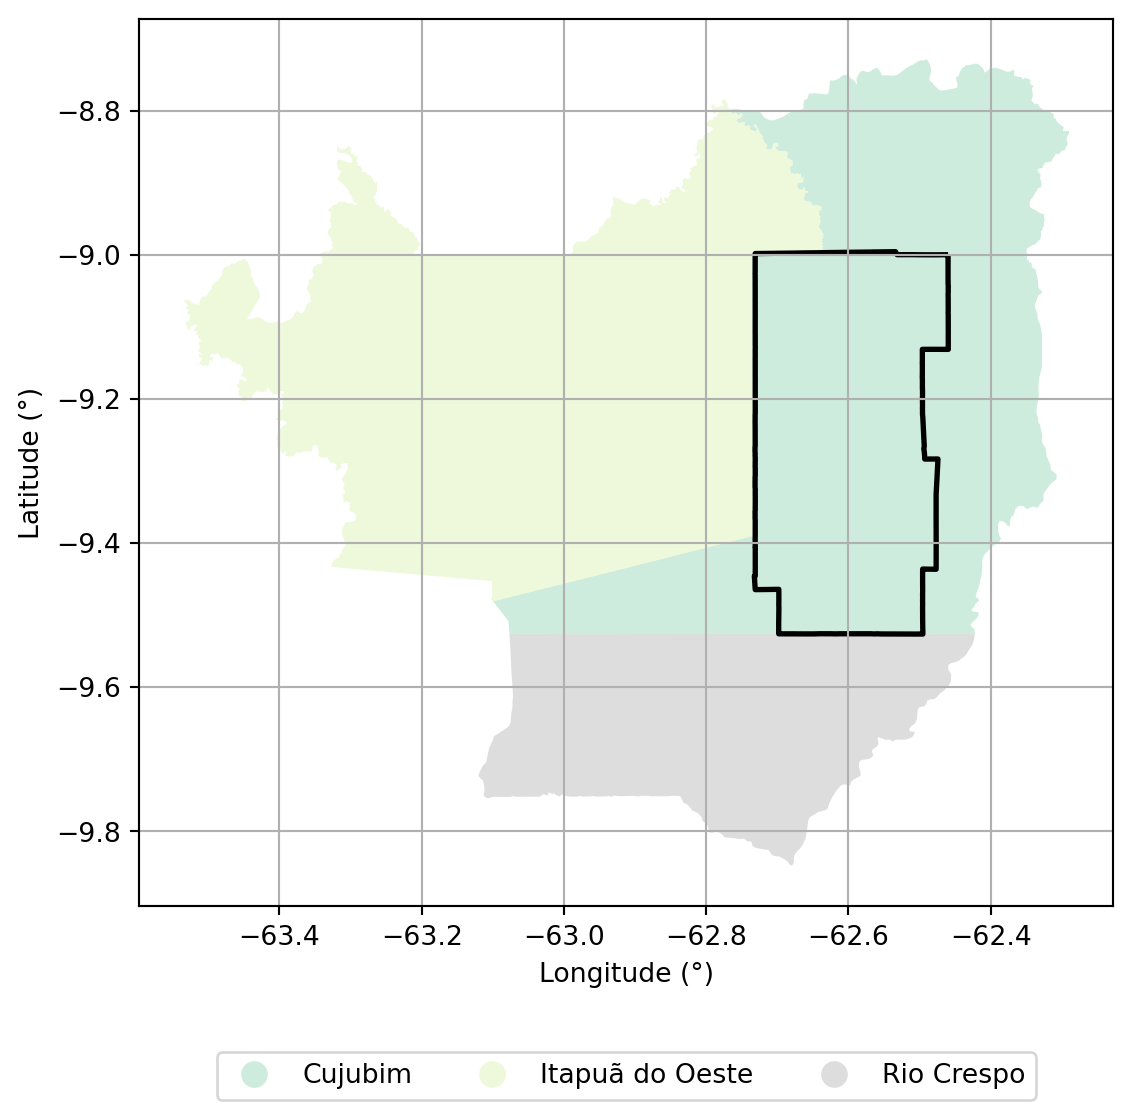
\includegraphics{xx-analise-individual-modelo_files/figure-pdf/cell-3-output-4.pdf}

\n  

\n    

\n      

Código da UF

\n      

Estado

\n      

UF

\n      

Código do Município

\n      

Nome do Município

\n    

\n  

\n  

\n    

\n      

12.0000

\n      

Acre

\n      

AC

\n      

1200302

\n      

Feijó

\n    

\n    

\n      

12.0000

\n      

Acre

\n      

AC

\n      

1200344

\n      

Manoel Urbano

\n    

\n  

\n

\subsubsection{Unidades de
Conservação}\label{unidades-de-conservauxe7uxe3o}

Não há sobreposição

\subsubsection{Terras Indígenas}\label{terras-induxedgenas}

Não há sobreposição

\subsubsection{Projetos de Assentamento}\label{projetos-de-assentamento}

Não há sobreposição

\subsubsection{Território Quilombola}\label{territuxf3rio-quilombola}

Não há sobreposição

\subsubsection{SIGEF}\label{sigef}

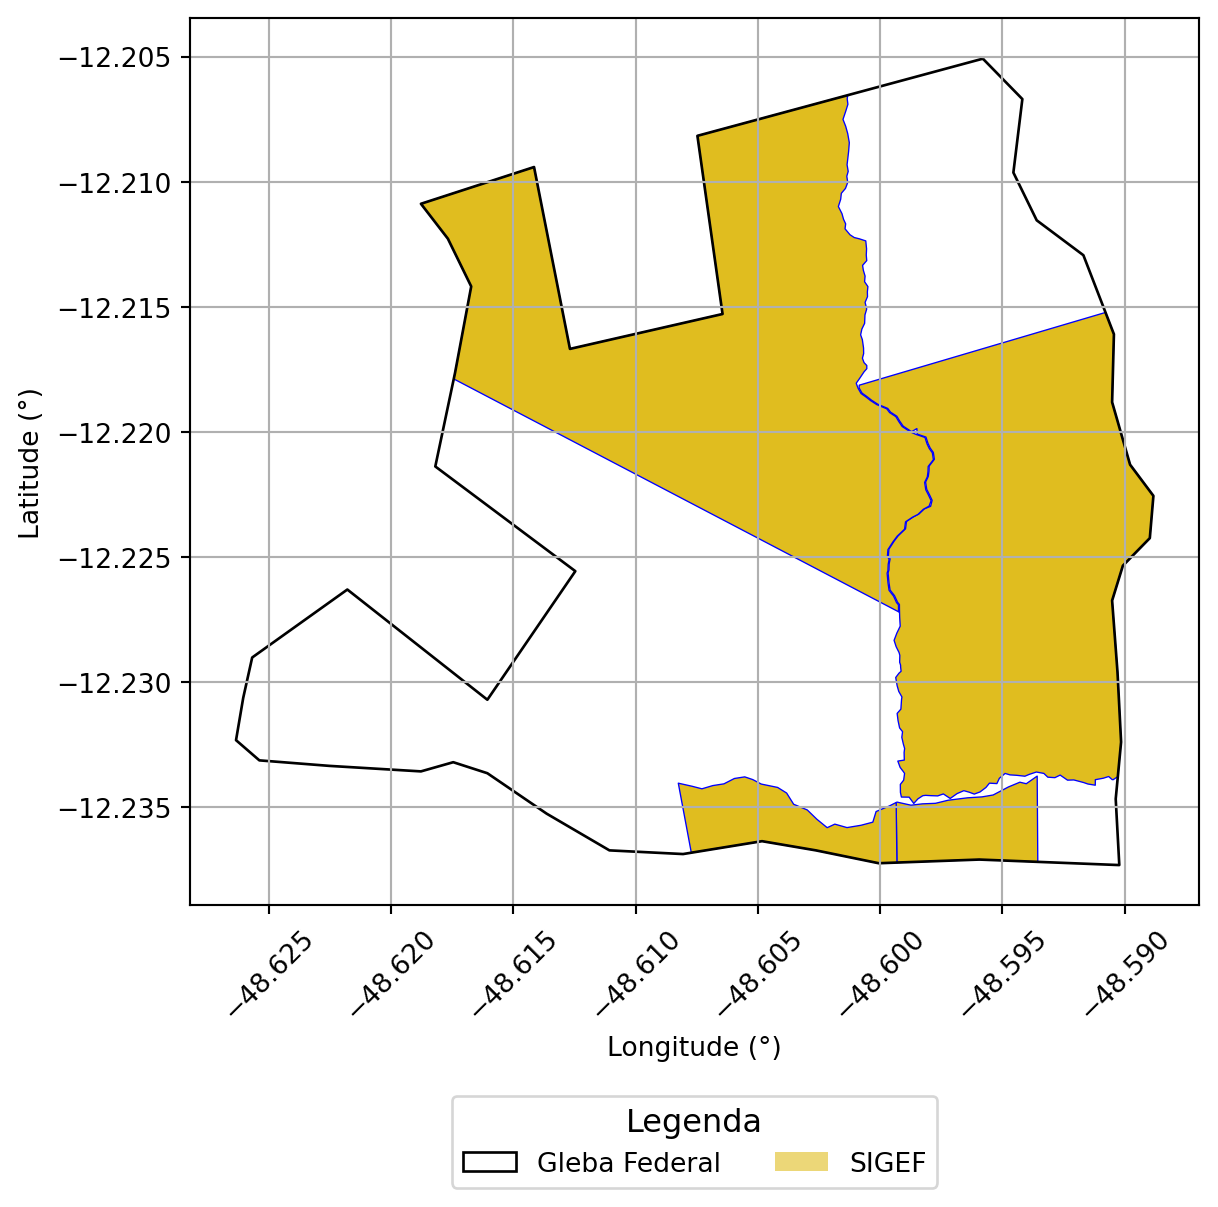
\includegraphics{xx-analise-individual-modelo_files/figure-pdf/cell-3-output-15.pdf}

\n  

\n    

\n      

Código SIGEF

\n      

Natureza do Polígono

\n      

Área Sobreposta (ha)

\n    

\n  

\n  

\n    

\n      

634d365d-2fbb-4e89-895d-7287c0dd3e77

\n      

Particular

\n      

124.7446

\n    

\n    

\n      

e58b01a6-e455-43aa-9b7b-7153796c384a

\n      

Particular

\n      

132.4867

\n    

\n    

\n      

bd3d45e0-6fb8-4080-8640-59156cdeca7a

\n      

Particular

\n      

59.6182

\n    

\n    

\n      

8c669355-5004-4be7-83cc-da7ce2f92f39

\n      

Particular

\n      

172.4033

\n    

\n    

\n      

e93433ee-22ec-4297-a86e-7a918ac609ac

\n      

Particular

\n      

56.6682

\n    

\n    

\n      

839ffc79-4878-487a-a5fa-a134f8cc644b

\n      

Particular

\n      

54.4402

\n    

\n    

\n      

760bd52e-f140-4f5c-acef-db8ad507a21e

\n      

Particular

\n      

0.2447

\n    

\n    

\n      

c7dfca7e-be66-456d-b298-bbb9f9c06de5

\n      

Particular

\n      

159.8261

\n    

\n    

\n      

ecb0d436-734c-4d6a-8b47-0b1e9ef2e394

\n      

Particular

\n      

149.2334

\n    

\n    

\n      

5ec05159-4656-485e-8f7b-8441cf377b43

\n      

Particular

\n      

82.9672

\n    

\n    

\n      

1fb89f89-0e2a-4192-8176-200d6764ce40

\n      

Particular

\n      

129.3393

\n    

\n    

\n      

a0defbdb-e4cd-4e75-a3df-70dde1ad329e

\n      

Particular

\n      

120.1032

\n    

\n    

\n      

74f9f09f-909e-44c5-822d-2725dfb029e0

\n      

Particular

\n      

122.1359

\n    

\n    

\n      

e3fb5282-6d45-4279-9cd4-7111e8d61aa1

\n      

Particular

\n      

220.6357

\n    

\n    

\n      

7ffd2c52-cefd-4d0d-9488-f28ca50f3c29

\n      

Particular

\n      

86.3175

\n    

\n    

\n      

bca3239a-ce98-4488-a99a-41d9a3a3bf37

\n      

Particular

\n      

195.5084

\n    

\n    

\n      

41af1f06-2521-440d-9e85-89a31effcdd4

\n      

Particular

\n      

124.8105

\n    

\n    

\n      

6ff4d949-0688-49c6-a20a-7df80a229c51

\n      

Particular

\n      

95.3128

\n    

\n    

\n      

c11a39f0-76f5-40d7-b46e-9e0907478c11

\n      

Particular

\n      

148.0050

\n    

\n    

\n      

347d2aab-c505-41e0-b505-201d148f0ca0

\n      

Particular

\n      

145.4595

\n    

\n    

\n      

1c61e63c-d146-4475-8bb8-207d6904cd4e

\n      

Particular

\n      

156.5960

\n    

\n  

\n

\subsubsection{SNCI}\label{snci}

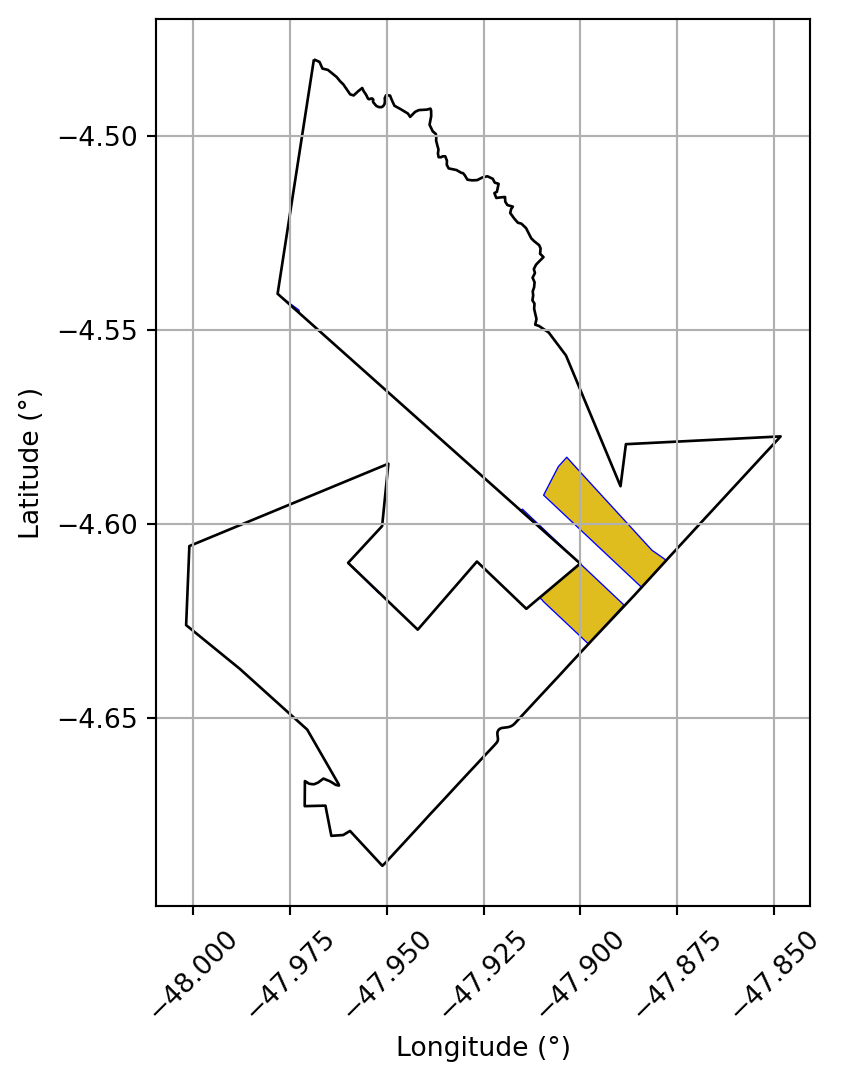
\includegraphics{xx-analise-individual-modelo_files/figure-pdf/cell-3-output-18.pdf}

\n  

\n    

\n      

Código SNCI

\n      

Área Sobreposta (ha)

\n    

\n  

\n  

\n    

\n      

141701000001-70

\n      

2544.5339

\n    

\n  

\n

\subsection{Gleba Analisada: AFLUENTE - PARTE
A3}\label{gleba-analisada-afluente---parte-a3}

\n  

\n    

\n      

Nome da Gleba

\n      

Área (ha)

\n    

\n  

\n  

\n    

\n      

AFLUENTE - PARTE A3

\n      

5054.4736

\n    

\n  

\n

\subsubsection{Abrangência Municipal}\label{abranguxeancia-municipal-1}

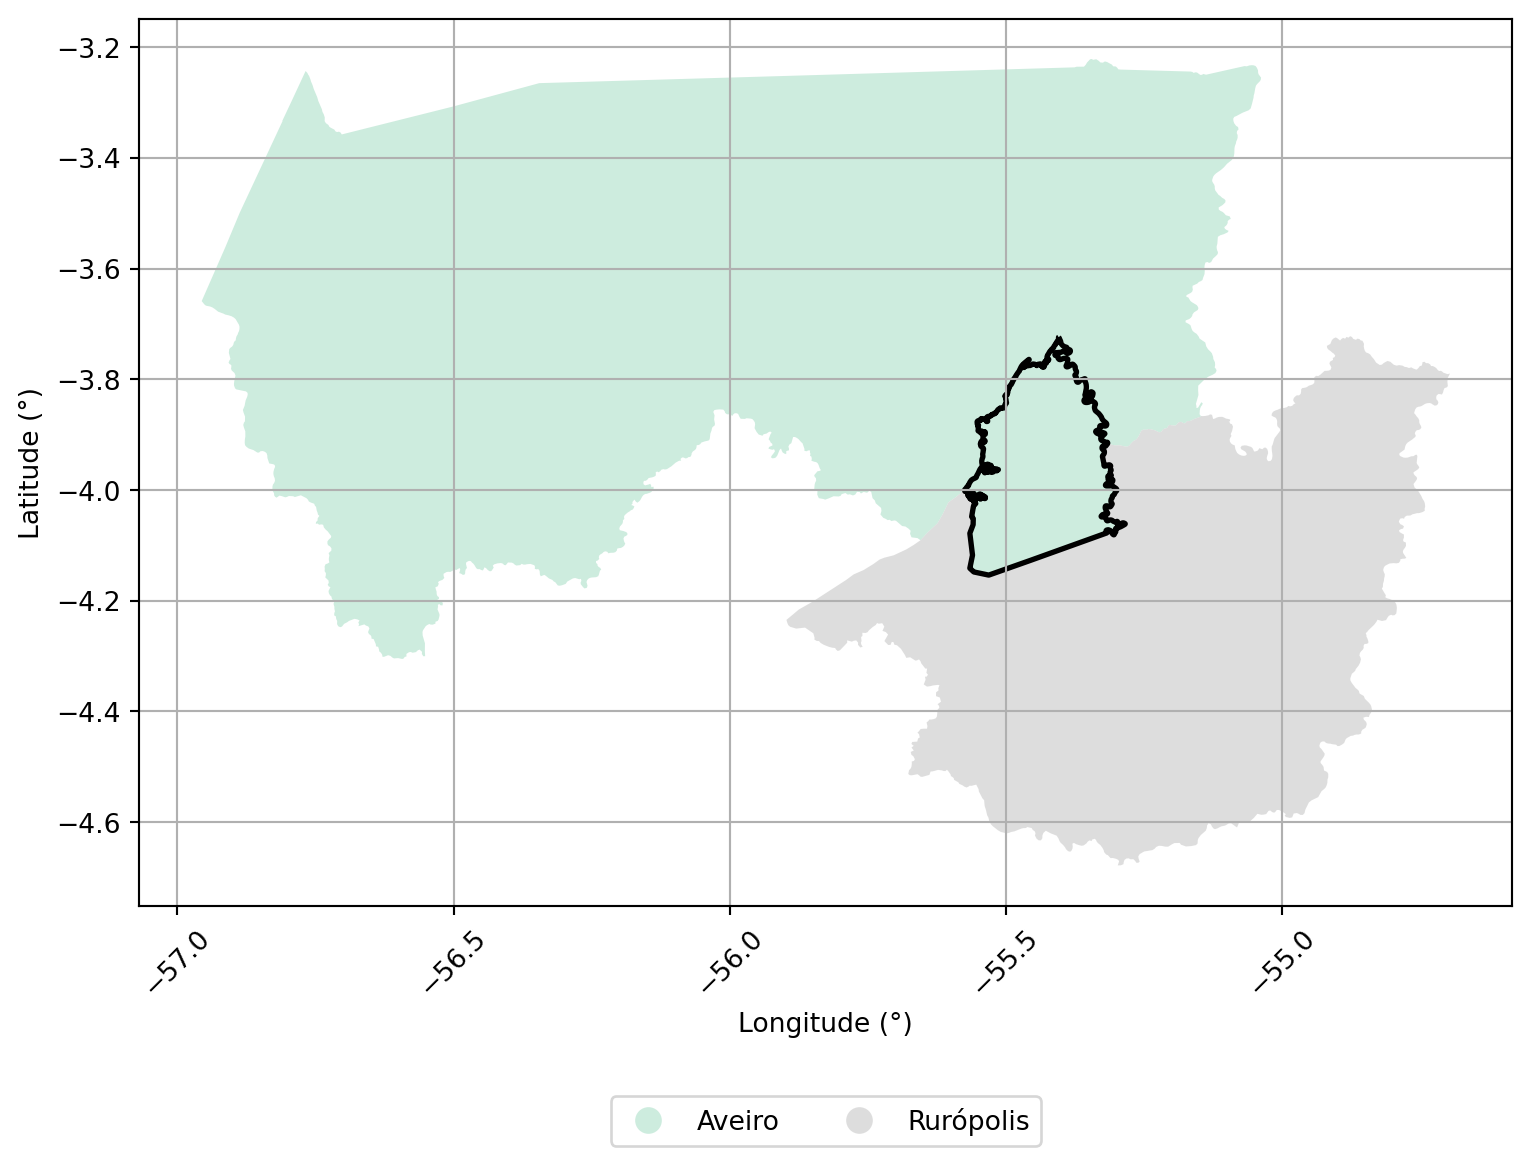
\includegraphics{xx-analise-individual-modelo_files/figure-pdf/cell-3-output-23.pdf}

\n  

\n    

\n      

Código da UF

\n      

Estado

\n      

UF

\n      

Código do Município

\n      

Nome do Município

\n    

\n  

\n  

\n    

\n      

12.0000

\n      

Acre

\n      

AC

\n      

1200302

\n      

Feijó

\n    

\n    

\n      

12.0000

\n      

Acre

\n      

AC

\n      

1200344

\n      

Manoel Urbano

\n    

\n  

\n

\subsubsection{Unidades de
Conservação}\label{unidades-de-conservauxe7uxe3o-1}

Não há sobreposição

\subsubsection{Terras Indígenas}\label{terras-induxedgenas-1}

Não há sobreposição

\subsubsection{Projetos de
Assentamento}\label{projetos-de-assentamento-1}

Não há sobreposição

\subsubsection{Território Quilombola}\label{territuxf3rio-quilombola-1}

Não há sobreposição

\subsubsection{SIGEF}\label{sigef-1}

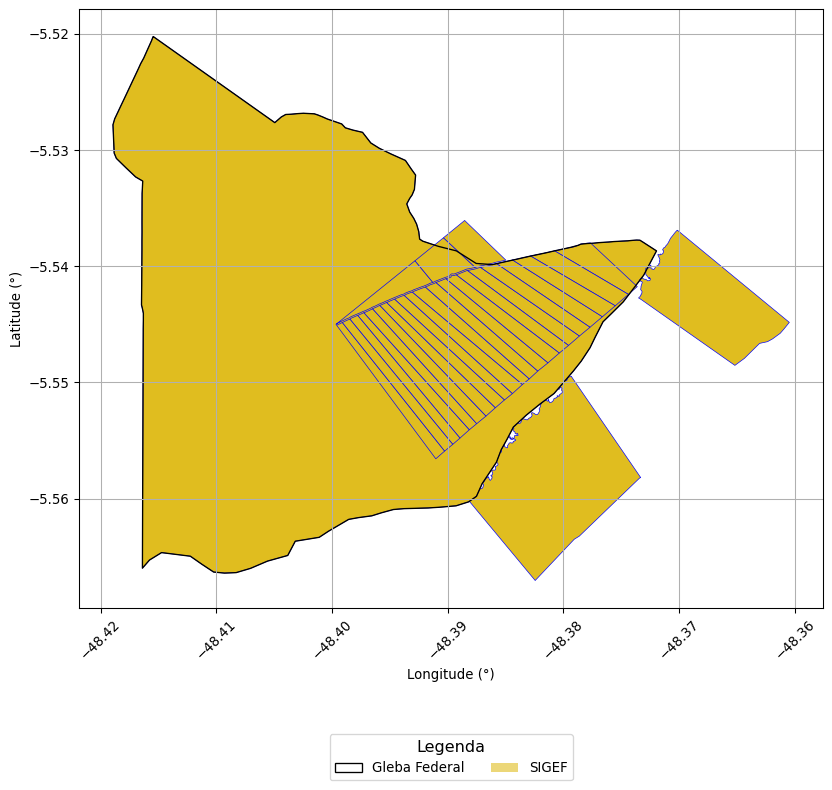
\includegraphics{xx-analise-individual-modelo_files/figure-pdf/cell-3-output-34.pdf}

\n  

\n    

\n      

Código SIGEF

\n      

Natureza do Polígono

\n      

Área Sobreposta (ha)

\n    

\n  

\n  

\n    

\n      

6ff4d949-0688-49c6-a20a-7df80a229c51

\n      

Particular

\n      

0.0000

\n    

\n    

\n      

41af1f06-2521-440d-9e85-89a31effcdd4

\n      

Particular

\n      

0.0000

\n    

\n    

\n      

bca3239a-ce98-4488-a99a-41d9a3a3bf37

\n      

Particular

\n      

0.0000

\n    

\n    

\n      

e3fb5282-6d45-4279-9cd4-7111e8d61aa1

\n      

Particular

\n      

0.0004

\n    

\n    

\n      

a0defbdb-e4cd-4e75-a3df-70dde1ad329e

\n      

Particular

\n      

0.0001

\n    

\n    

\n      

347d2aab-c505-41e0-b505-201d148f0ca0

\n      

Particular

\n      

0.0001

\n    

\n    

\n      

ecb0d436-734c-4d6a-8b47-0b1e9ef2e394

\n      

Particular

\n      

0.0000

\n    

\n    

\n      

57e38e6f-4306-4baa-8224-97185df5c6f2

\n      

Particular

\n      

73.3319

\n    

\n    

\n      

7ea7456a-59d7-43be-854a-9eb7192b6fa2

\n      

Particular

\n      

173.4258

\n    

\n    

\n      

bd3d45e0-6fb8-4080-8640-59156cdeca7a

\n      

Particular

\n      

0.0001

\n    

\n    

\n      

5ec05159-4656-485e-8f7b-8441cf377b43

\n      

Particular

\n      

0.0001

\n    

\n  

\n

\subsubsection{SNCI}\label{snci-1}

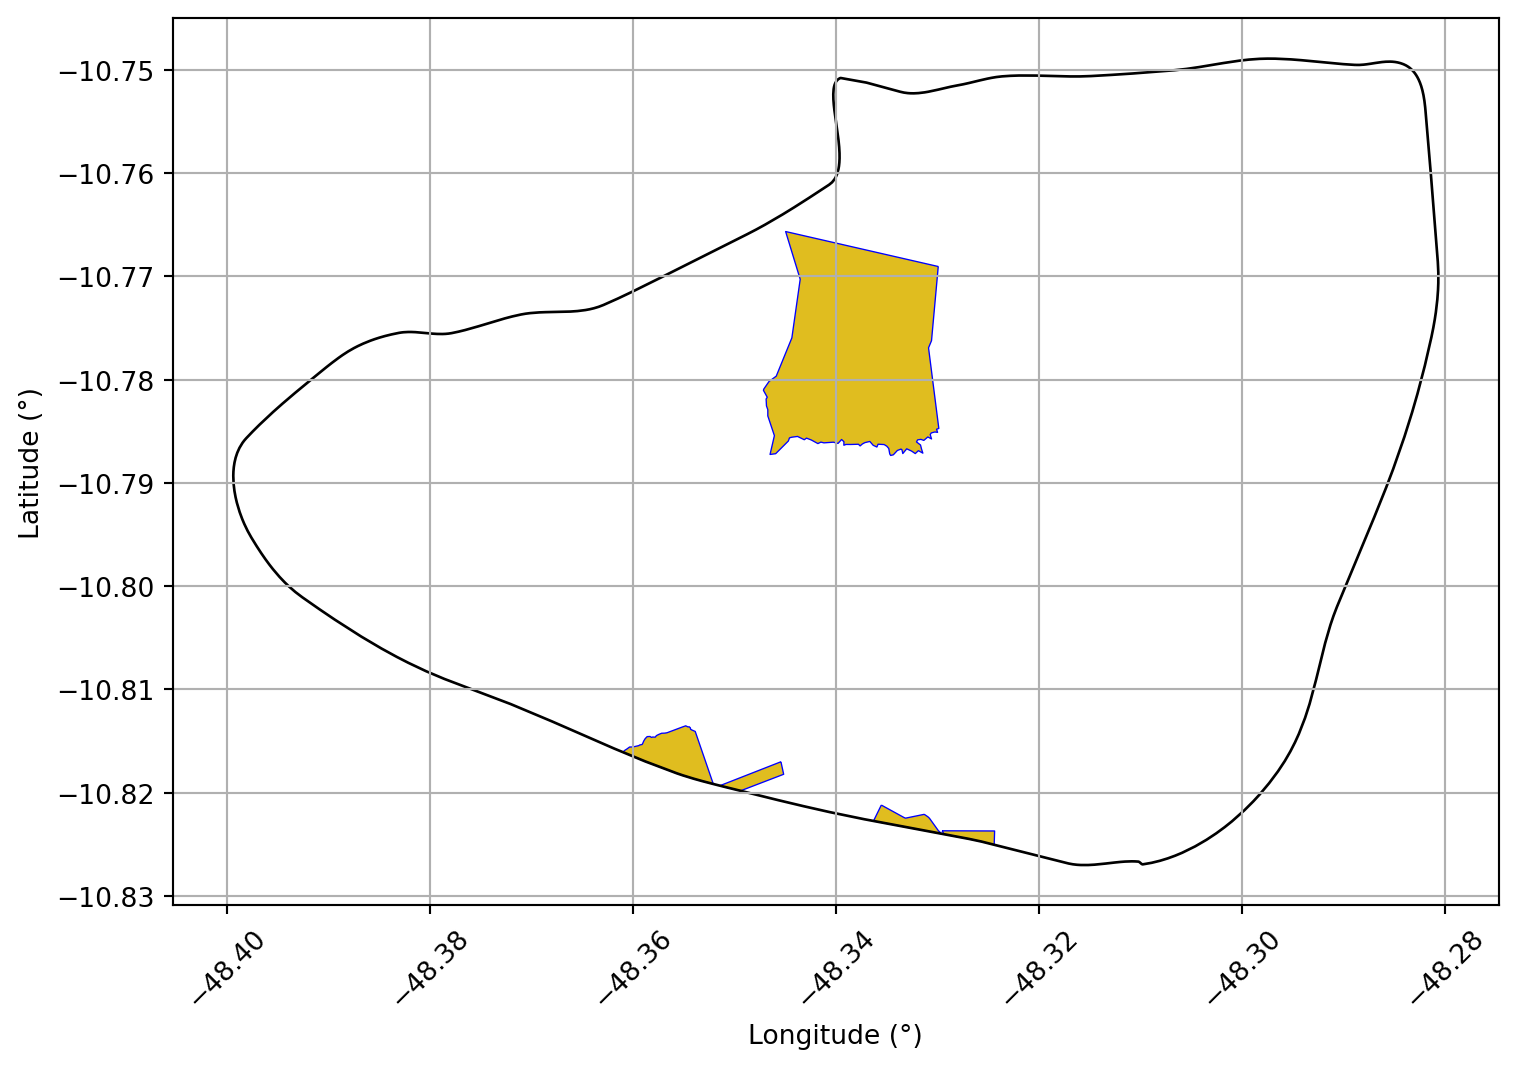
\includegraphics{xx-analise-individual-modelo_files/figure-pdf/cell-3-output-37.pdf}

\n  

\n    

\n      

Código SNCI

\n      

Área Sobreposta (ha)

\n    

\n  

\n  

\n    

\n      

141701000002-51

\n      

5244.5998

\n    

\n  

\n

\subsection{Gleba Analisada: AFLUENTE - PARTE B2 -
REMANESCENTE}\label{gleba-analisada-afluente---parte-b2---remanescente}

\n  

\n    

\n      

Nome da Gleba

\n      

Área (ha)

\n    

\n  

\n  

\n    

\n      

AFLUENTE - PARTE B2 - REMANESCENTE

\n      

5448.3825

\n    

\n  

\n

\subsubsection{Abrangência Municipal}\label{abranguxeancia-municipal-2}

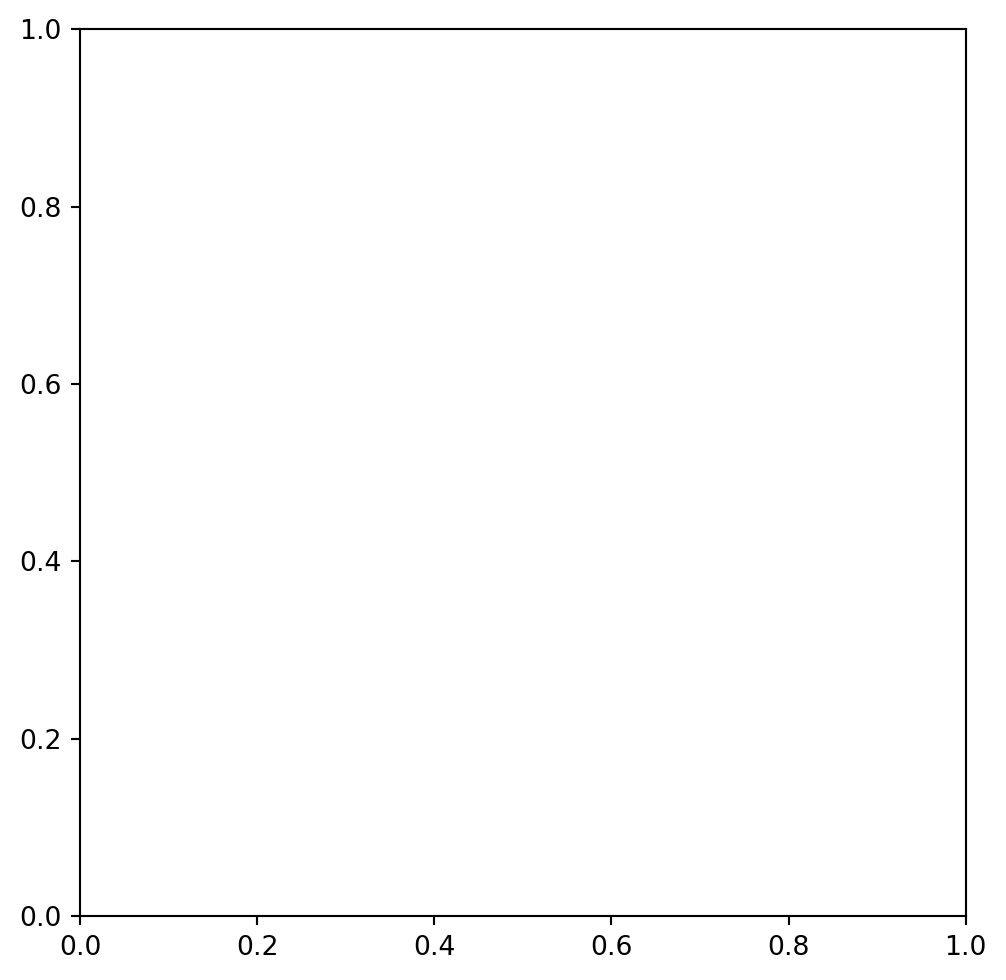
\includegraphics{xx-analise-individual-modelo_files/figure-pdf/cell-3-output-42.pdf}

\n  

\n    

\n      

Código da UF

\n      

Estado

\n      

UF

\n      

Código do Município

\n      

Nome do Município

\n    

\n  

\n  

\n    

\n      

12.0000

\n      

Acre

\n      

AC

\n      

1200302

\n      

Feijó

\n    

\n    

\n      

12.0000

\n      

Acre

\n      

AC

\n      

1200344

\n      

Manoel Urbano

\n    

\n  

\n

\subsubsection{Unidades de
Conservação}\label{unidades-de-conservauxe7uxe3o-2}

Não há sobreposição

\subsubsection{Terras Indígenas}\label{terras-induxedgenas-2}

Não há sobreposição

\subsubsection{Projetos de
Assentamento}\label{projetos-de-assentamento-2}

Não há sobreposição

\subsubsection{Território Quilombola}\label{territuxf3rio-quilombola-2}

Não há sobreposição

\subsubsection{SIGEF}\label{sigef-2}

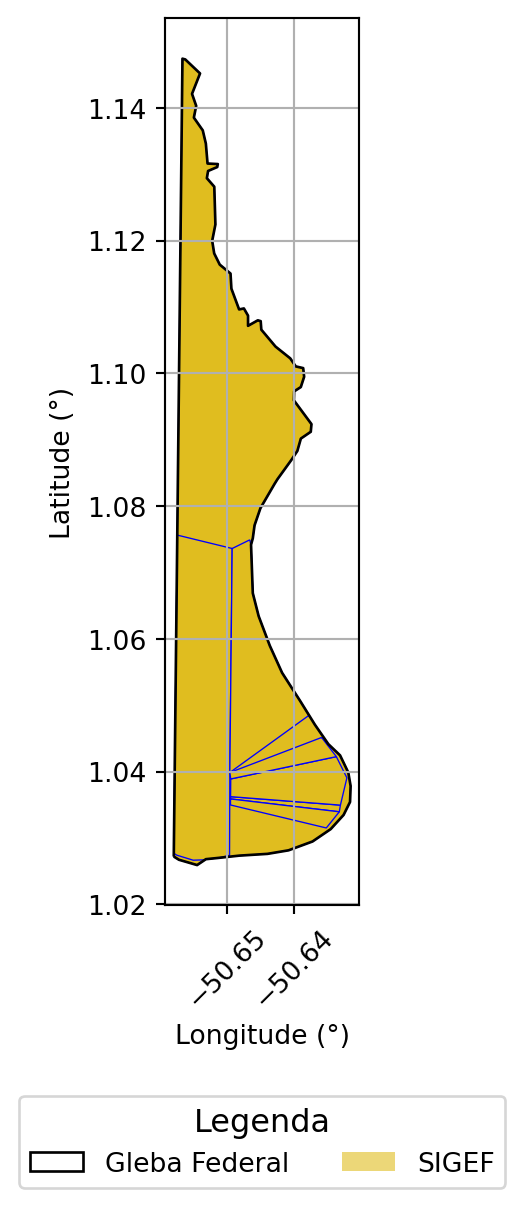
\includegraphics{xx-analise-individual-modelo_files/figure-pdf/cell-3-output-53.pdf}

\n  

\n    

\n      

Código SIGEF

\n      

Natureza do Polígono

\n      

Área Sobreposta (ha)

\n    

\n  

\n  

\n    

\n      

ed387024-014b-45c4-beab-6b5a623420a9

\n      

Particular

\n      

100.9471

\n    

\n    

\n      

05cd5fd0-417a-4f28-90c8-96ac36a06c33

\n      

Particular

\n      

103.2579

\n    

\n    

\n      

22ae4da6-1f18-4537-97b5-f9d3d83d5c4c

\n      

Particular

\n      

102.2345

\n    

\n    

\n      

6a536291-52ef-44cf-82e2-a90cf478f063

\n      

Particular

\n      

163.8424

\n    

\n    

\n      

ac69c7a4-41b6-48a1-b13c-150b553c13bd

\n      

Particular

\n      

100.7934

\n    

\n    

\n      

6ff83f63-8450-4b09-b793-d3853f1991a3

\n      

Particular

\n      

156.4022

\n    

\n    

\n      

a7bef773-0429-4566-8a0b-3c52005c3dbc

\n      

Particular

\n      

100.6599

\n    

\n    

\n      

694e2de7-b643-4b23-b845-748a4f357e7e

\n      

Particular

\n      

160.3402

\n    

\n    

\n      

411bc08e-48f7-4a7b-a5c6-98c2a2594432

\n      

Particular

\n      

97.5246

\n    

\n    

\n      

ccbea799-f792-414f-979d-c466639d8a11

\n      

Particular

\n      

333.1174

\n    

\n    

\n      

8259b99c-356f-401a-8a8b-52587f1daf1b

\n      

Particular

\n      

119.2588

\n    

\n    

\n      

953f2174-46bc-4f18-bca5-1cf72de5ce04

\n      

Particular

\n      

103.4228

\n    

\n    

\n      

9fd6c027-d7bf-403a-b219-f6521bf68d38

\n      

Particular

\n      

117.2801

\n    

\n    

\n      

3a84dcc2-310e-45c6-886c-95a5e157891d

\n      

Particular

\n      

59.0766

\n    

\n    

\n      

416ac40d-421f-4654-a518-ad8f51fced05

\n      

Particular

\n      

98.0219

\n    

\n    

\n      

b8f2b04d-45a5-4ba8-b9ef-94f78e6a1a60

\n      

Particular

\n      

55.4071

\n    

\n    

\n      

78a7b8e3-da21-4fb2-8f74-d511280c8637

\n      

Particular

\n      

89.2791

\n    

\n    

\n      

f9d37f50-78fa-4fe2-b198-235a115ad918

\n      

Particular

\n      

96.8585

\n    

\n    

\n      

fc1b3f65-ed49-459f-9acb-fdd542b0f8f4

\n      

Particular

\n      

109.2407

\n    

\n    

\n      

2ac504ca-842b-4263-b119-f4dae5766086

\n      

Particular

\n      

126.4301

\n    

\n    

\n      

b664ed45-3b7a-45e4-b5c2-caaffad7b342

\n      

Particular

\n      

455.4490

\n    

\n    

\n      

8a9929c8-753e-4d3d-9c05-158f6bad8f37

\n      

Particular

\n      

168.5496

\n    

\n    

\n      

ea5f5858-31aa-4533-b8c8-37ddddab8708

\n      

Particular

\n      

134.8613

\n    

\n    

\n      

760bd52e-f140-4f5c-acef-db8ad507a21e

\n      

Particular

\n      

268.4476

\n    

\n    

\n      

839ffc79-4878-487a-a5fa-a134f8cc644b

\n      

Particular

\n      

108.7053

\n    

\n    

\n      

e93433ee-22ec-4297-a86e-7a918ac609ac

\n      

Particular

\n      

68.2546

\n    

\n    

\n      

8c669355-5004-4be7-83cc-da7ce2f92f39

\n      

Particular

\n      

105.8609

\n    

\n    

\n      

bd3d45e0-6fb8-4080-8640-59156cdeca7a

\n      

Particular

\n      

33.7565

\n    

\n    

\n      

e58b01a6-e455-43aa-9b7b-7153796c384a

\n      

Particular

\n      

31.4751

\n    

\n    

\n      

5ec05159-4656-485e-8f7b-8441cf377b43

\n      

Particular

\n      

11.6960

\n    

\n    

\n      

e81e387f-4218-4176-91b2-de38cf8f779d

\n      

Particular

\n      

180.7211

\n    

\n    

\n      

b64a1397-350d-402a-88e2-28a9c21a46bf

\n      

Particular

\n      

117.6915

\n    

\n    

\n      

2d6702a5-b682-4d13-a2d1-6a48d2fcb5b3

\n      

Particular

\n      

362.6850

\n    

\n    

\n      

60dd1c47-78d5-4470-aba0-825a6e7b3eb4

\n      

Particular

\n      

139.7083

\n    

\n    

\n      

14fe4b46-1630-4448-8e4c-0163626f4482

\n      

Particular

\n      

101.5369

\n    

\n    

\n      

05fb2842-50a2-45cc-97e2-b7ab8776c6ee

\n      

Particular

\n      

59.2423

\n    

\n    

\n      

edb0d8da-cb65-45cc-90c6-4b3372e17589

\n      

Particular

\n      

102.9616

\n    

\n  

\n

\subsubsection{SNCI}\label{snci-2}

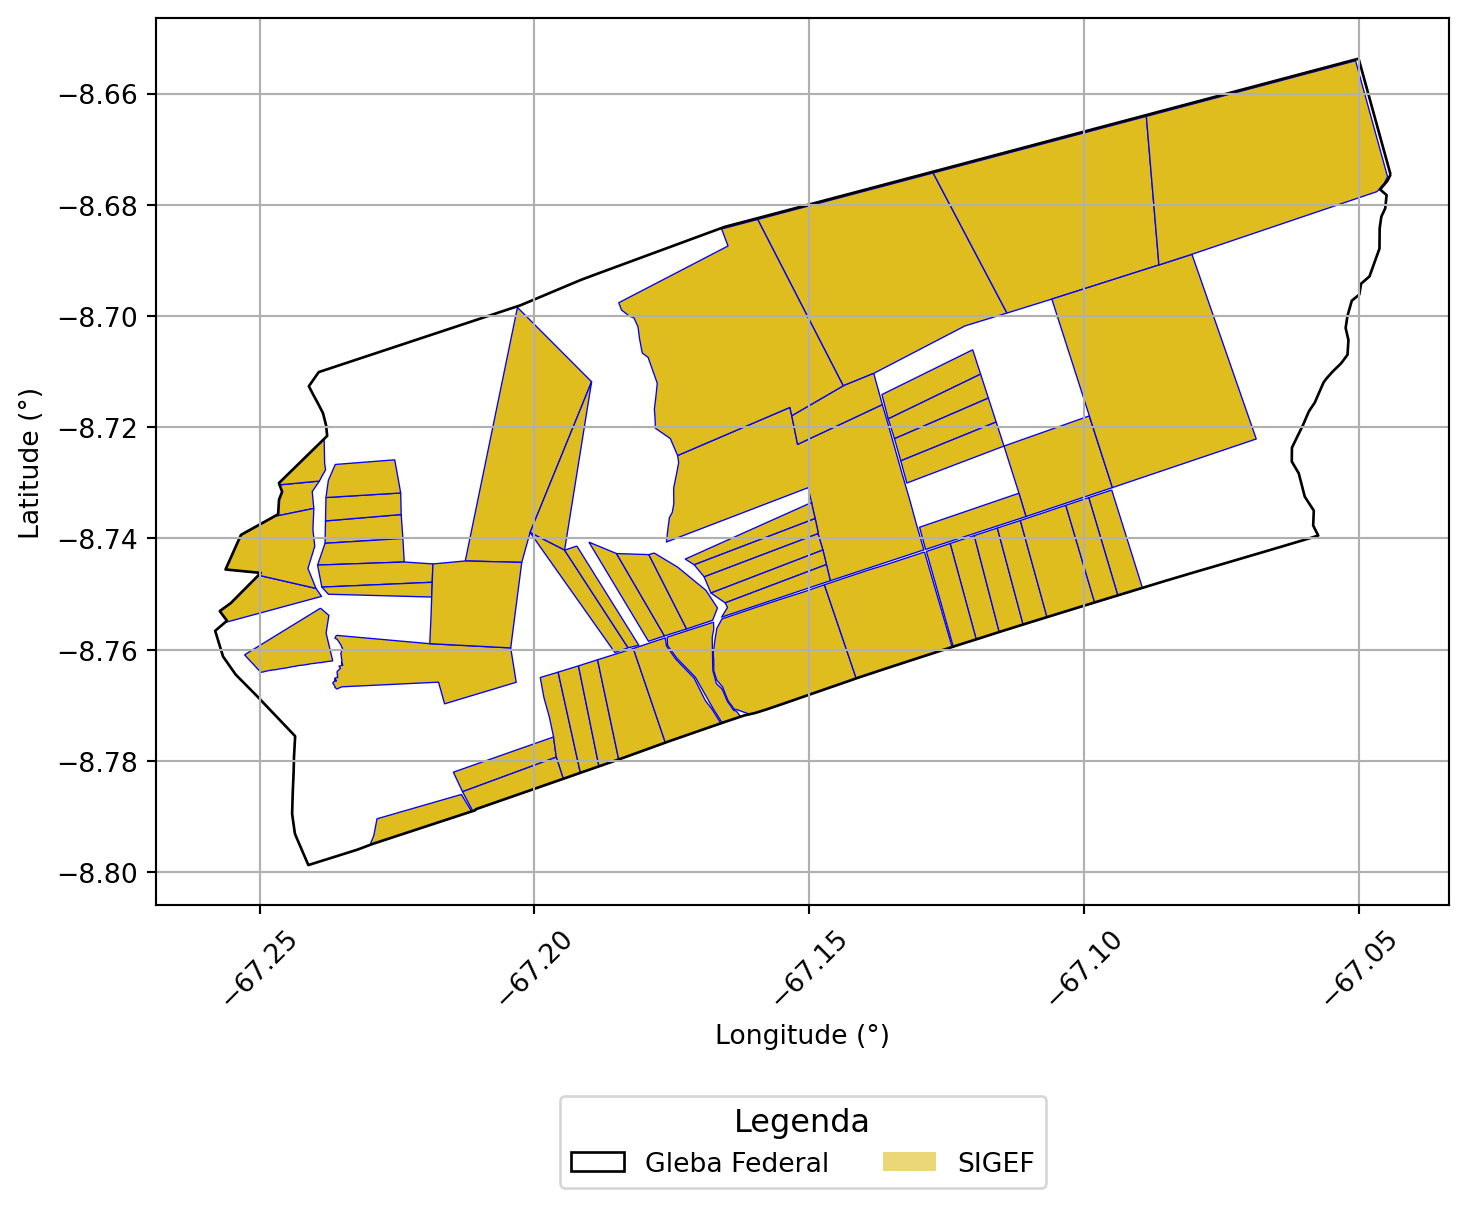
\includegraphics{xx-analise-individual-modelo_files/figure-pdf/cell-3-output-56.pdf}

\n  

\n    

\n      

Código SNCI

\n      

Área Sobreposta (ha)

\n    

\n  

\n  

\n    

\n      

141611000003-76

\n      

5649.9940

\n    

\n  

\n

\subsection{Gleba Analisada: AFLUENTE - PARTE
B3}\label{gleba-analisada-afluente---parte-b3}

\n  

\n    

\n      

Nome da Gleba

\n      

Área (ha)

\n    

\n  

\n  

\n    

\n      

AFLUENTE - PARTE B3

\n      

15342.5633

\n    

\n  

\n

\subsubsection{Abrangência Municipal}\label{abranguxeancia-municipal-3}

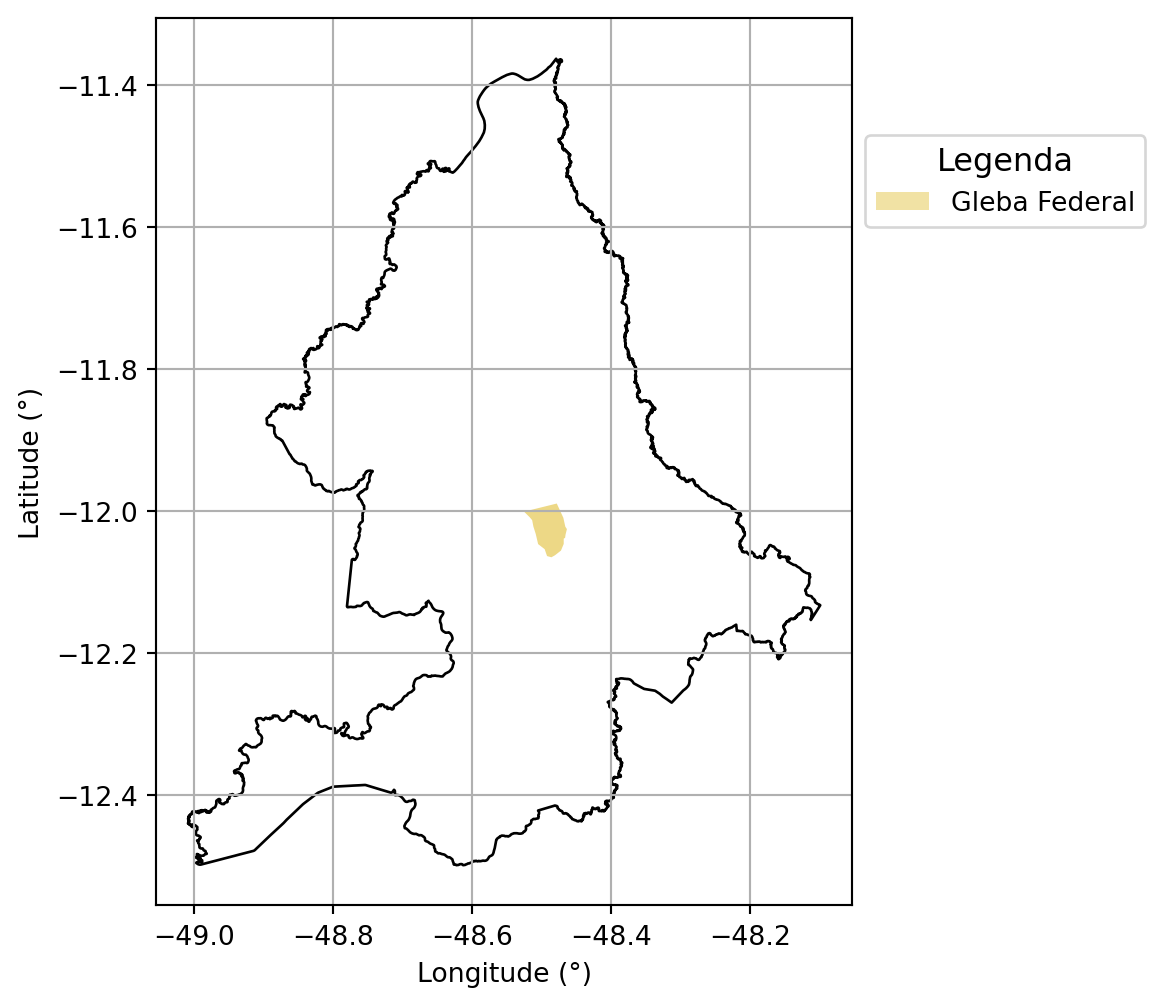
\includegraphics{xx-analise-individual-modelo_files/figure-pdf/cell-3-output-61.pdf}

\n  

\n    

\n      

Código da UF

\n      

Estado

\n      

UF

\n      

Código do Município

\n      

Nome do Município

\n    

\n  

\n  

\n    

\n      

12.0000

\n      

Acre

\n      

AC

\n      

1200302

\n      

Feijó

\n    

\n    

\n      

12.0000

\n      

Acre

\n      

AC

\n      

1200344

\n      

Manoel Urbano

\n    

\n  

\n

\subsubsection{Unidades de
Conservação}\label{unidades-de-conservauxe7uxe3o-3}

Não há sobreposição

\subsubsection{Terras Indígenas}\label{terras-induxedgenas-3}

Não há sobreposição

\subsubsection{Projetos de
Assentamento}\label{projetos-de-assentamento-3}

Não há sobreposição

\subsubsection{Território Quilombola}\label{territuxf3rio-quilombola-3}

Não há sobreposição

\subsubsection{SIGEF}\label{sigef-3}

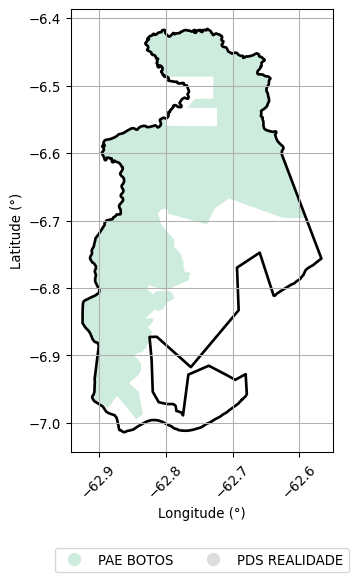
\includegraphics{xx-analise-individual-modelo_files/figure-pdf/cell-3-output-72.pdf}

\n  

\n    

\n      

Código SIGEF

\n      

Natureza do Polígono

\n      

Área Sobreposta (ha)

\n    

\n  

\n  

\n    

\n      

7f5a44d3-c9d0-4f0b-9caf-547a1d82f6de

\n      

Particular

\n      

201.8350

\n    

\n    

\n      

14fe4b46-1630-4448-8e4c-0163626f4482

\n      

Particular

\n      

0.0000

\n    

\n    

\n      

60dd1c47-78d5-4470-aba0-825a6e7b3eb4

\n      

Particular

\n      

0.0001

\n    

\n    

\n      

2d6702a5-b682-4d13-a2d1-6a48d2fcb5b3

\n      

Particular

\n      

0.0000

\n    

\n    

\n      

b64a1397-350d-402a-88e2-28a9c21a46bf

\n      

Particular

\n      

0.0000

\n    

\n    

\n      

e81e387f-4218-4176-91b2-de38cf8f779d

\n      

Particular

\n      

0.0000

\n    

\n    

\n      

5ec05159-4656-485e-8f7b-8441cf377b43

\n      

Particular

\n      

0.0000

\n    

\n    

\n      

e58b01a6-e455-43aa-9b7b-7153796c384a

\n      

Particular

\n      

0.0001

\n    

\n    

\n      

05cd5fd0-417a-4f28-90c8-96ac36a06c33

\n      

Particular

\n      

0.0002

\n    

\n    

\n      

bd3d45e0-6fb8-4080-8640-59156cdeca7a

\n      

Particular

\n      

0.0001

\n    

\n    

\n      

e93433ee-22ec-4297-a86e-7a918ac609ac

\n      

Particular

\n      

0.0001

\n    

\n    

\n      

839ffc79-4878-487a-a5fa-a134f8cc644b

\n      

Particular

\n      

0.0001

\n    

\n    

\n      

ea5f5858-31aa-4533-b8c8-37ddddab8708

\n      

Particular

\n      

0.0583

\n    

\n    

\n      

b664ed45-3b7a-45e4-b5c2-caaffad7b342

\n      

Particular

\n      

0.0001

\n    

\n    

\n      

7ea7456a-59d7-43be-854a-9eb7192b6fa2

\n      

Particular

\n      

19.0027

\n    

\n    

\n      

57e38e6f-4306-4baa-8224-97185df5c6f2

\n      

Particular

\n      

243.5564

\n    

\n    

\n      

1be351cf-bf96-4a4a-a7d1-402d21ca87d1

\n      

Particular

\n      

90.1921

\n    

\n    

\n      

8c669355-5004-4be7-83cc-da7ce2f92f39

\n      

Particular

\n      

0.0000

\n    

\n    

\n      

ccbea799-f792-414f-979d-c466639d8a11

\n      

Particular

\n      

0.0006

\n    

\n  

\n

\subsubsection{SNCI}\label{snci-3}

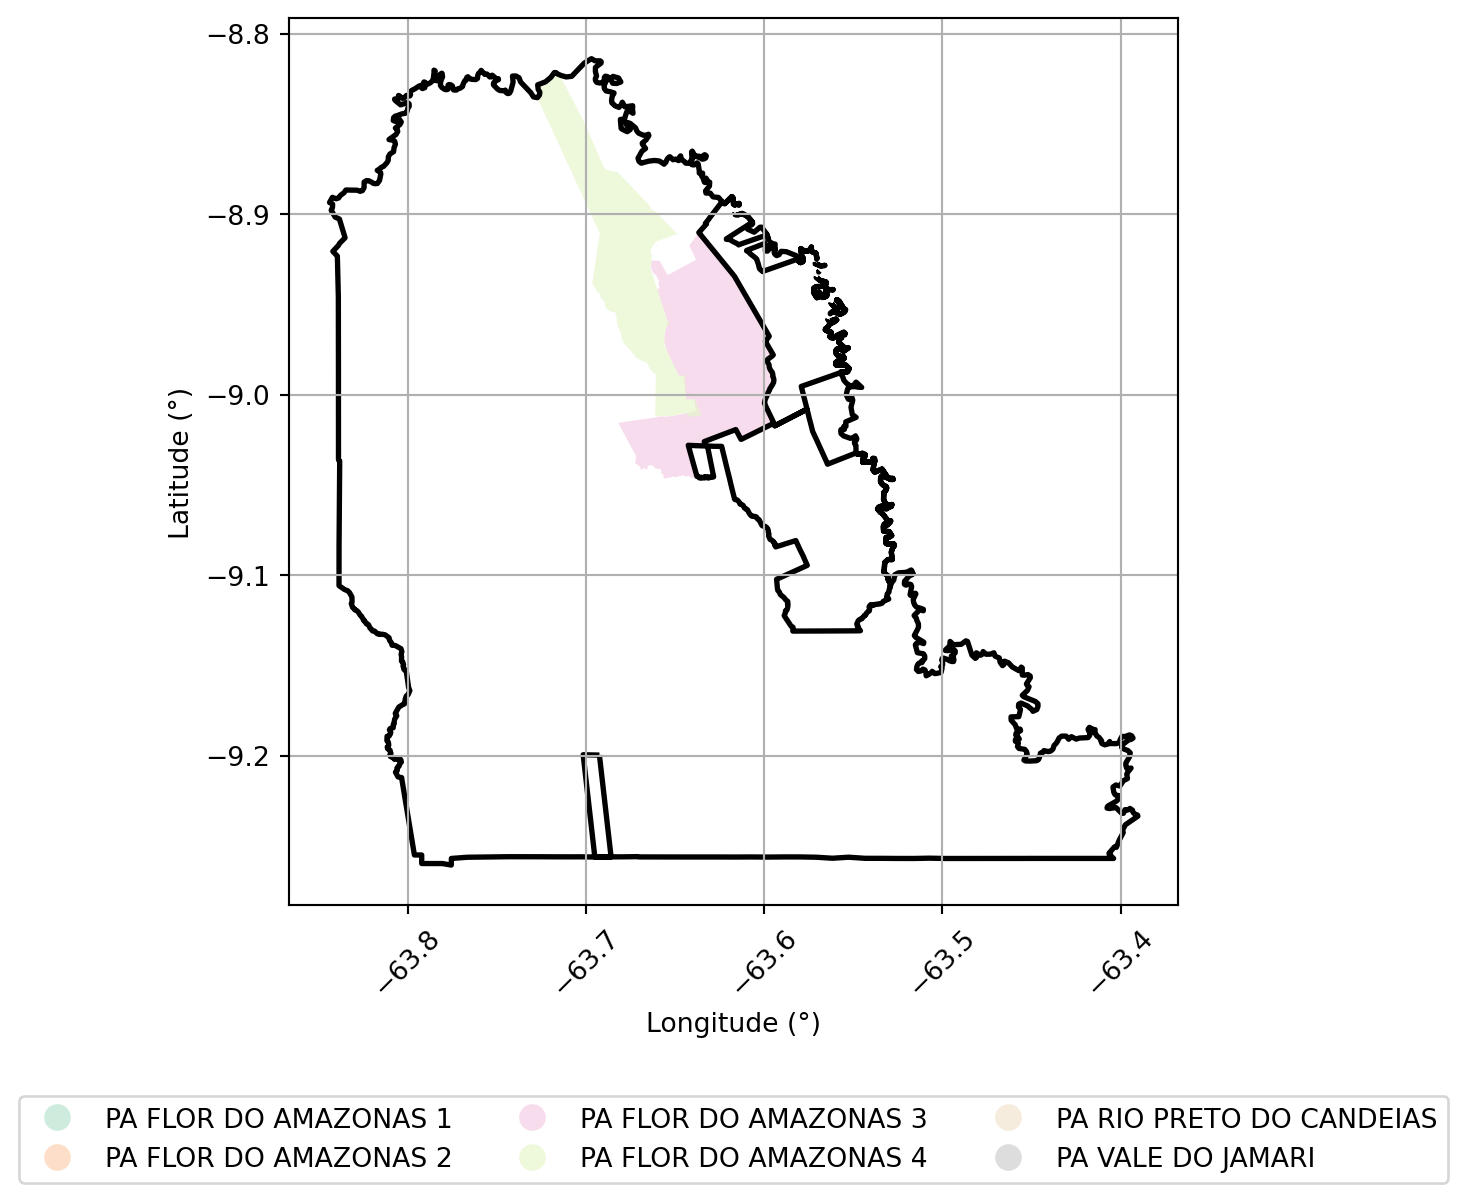
\includegraphics{xx-analise-individual-modelo_files/figure-pdf/cell-3-output-75.pdf}

\n  

\n    

\n      

Código SNCI

\n      

Área Sobreposta (ha)

\n    

\n  

\n  

\n    

\n      

140805000002-76

\n      

0.0001

\n    

\n    

\n      

141611000004-57

\n      

15914.4863

\n    

\n  

\n

\subsection{Gleba Analisada: AREZ PARTE A B E
C}\label{gleba-analisada-arez-parte-a-b-e-c}

\n  

\n    

\n      

Nome da Gleba

\n      

Área (ha)

\n    

\n  

\n  

\n    

\n      

AREZ PARTE A B E C

\n      

64572.9231

\n    

\n  

\n

\subsubsection{Abrangência Municipal}\label{abranguxeancia-municipal-4}

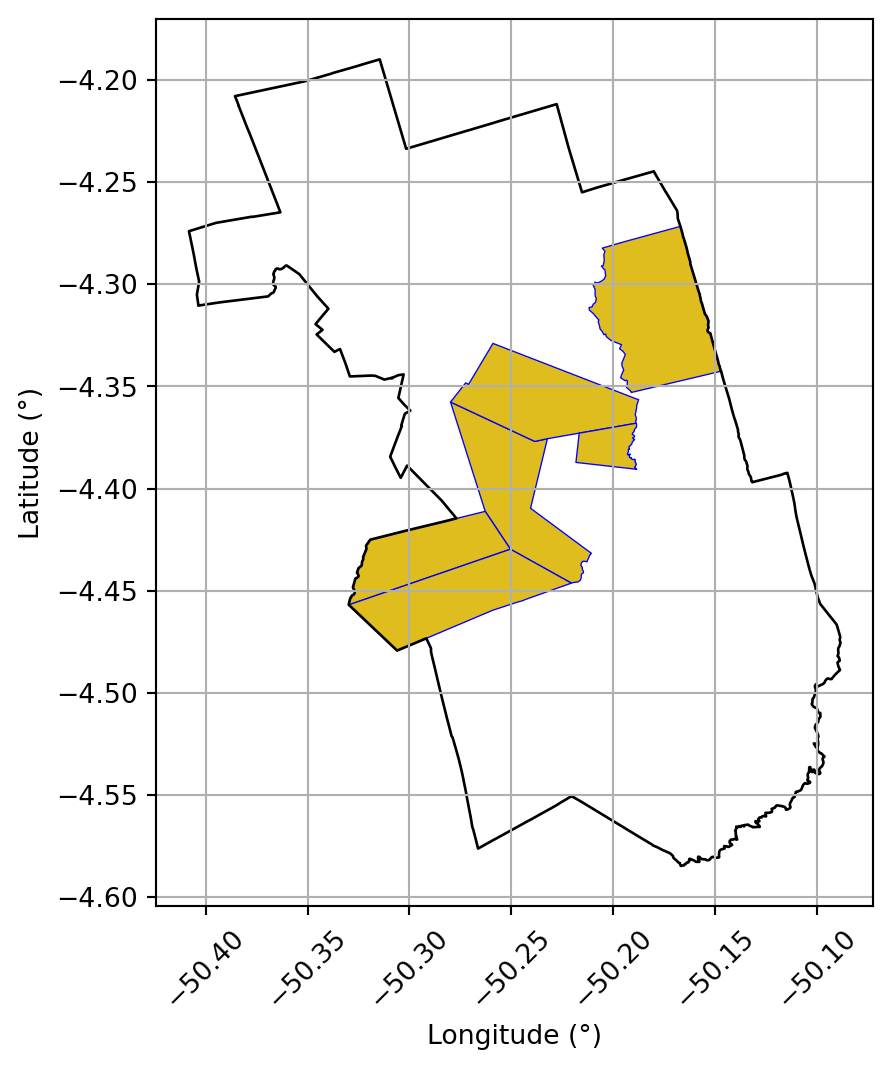
\includegraphics{xx-analise-individual-modelo_files/figure-pdf/cell-3-output-80.pdf}

\n  

\n    

\n      

Código da UF

\n      

Estado

\n      

UF

\n      

Código do Município

\n      

Nome do Município

\n    

\n  

\n  

\n    

\n      

12.0000

\n      

Acre

\n      

AC

\n      

1200344

\n      

Manoel Urbano

\n    

\n    

\n      

12.0000

\n      

Acre

\n      

AC

\n      

1200500

\n      

Sena Madureira

\n    

\n  

\n

\subsubsection{Unidades de
Conservação}\label{unidades-de-conservauxe7uxe3o-4}

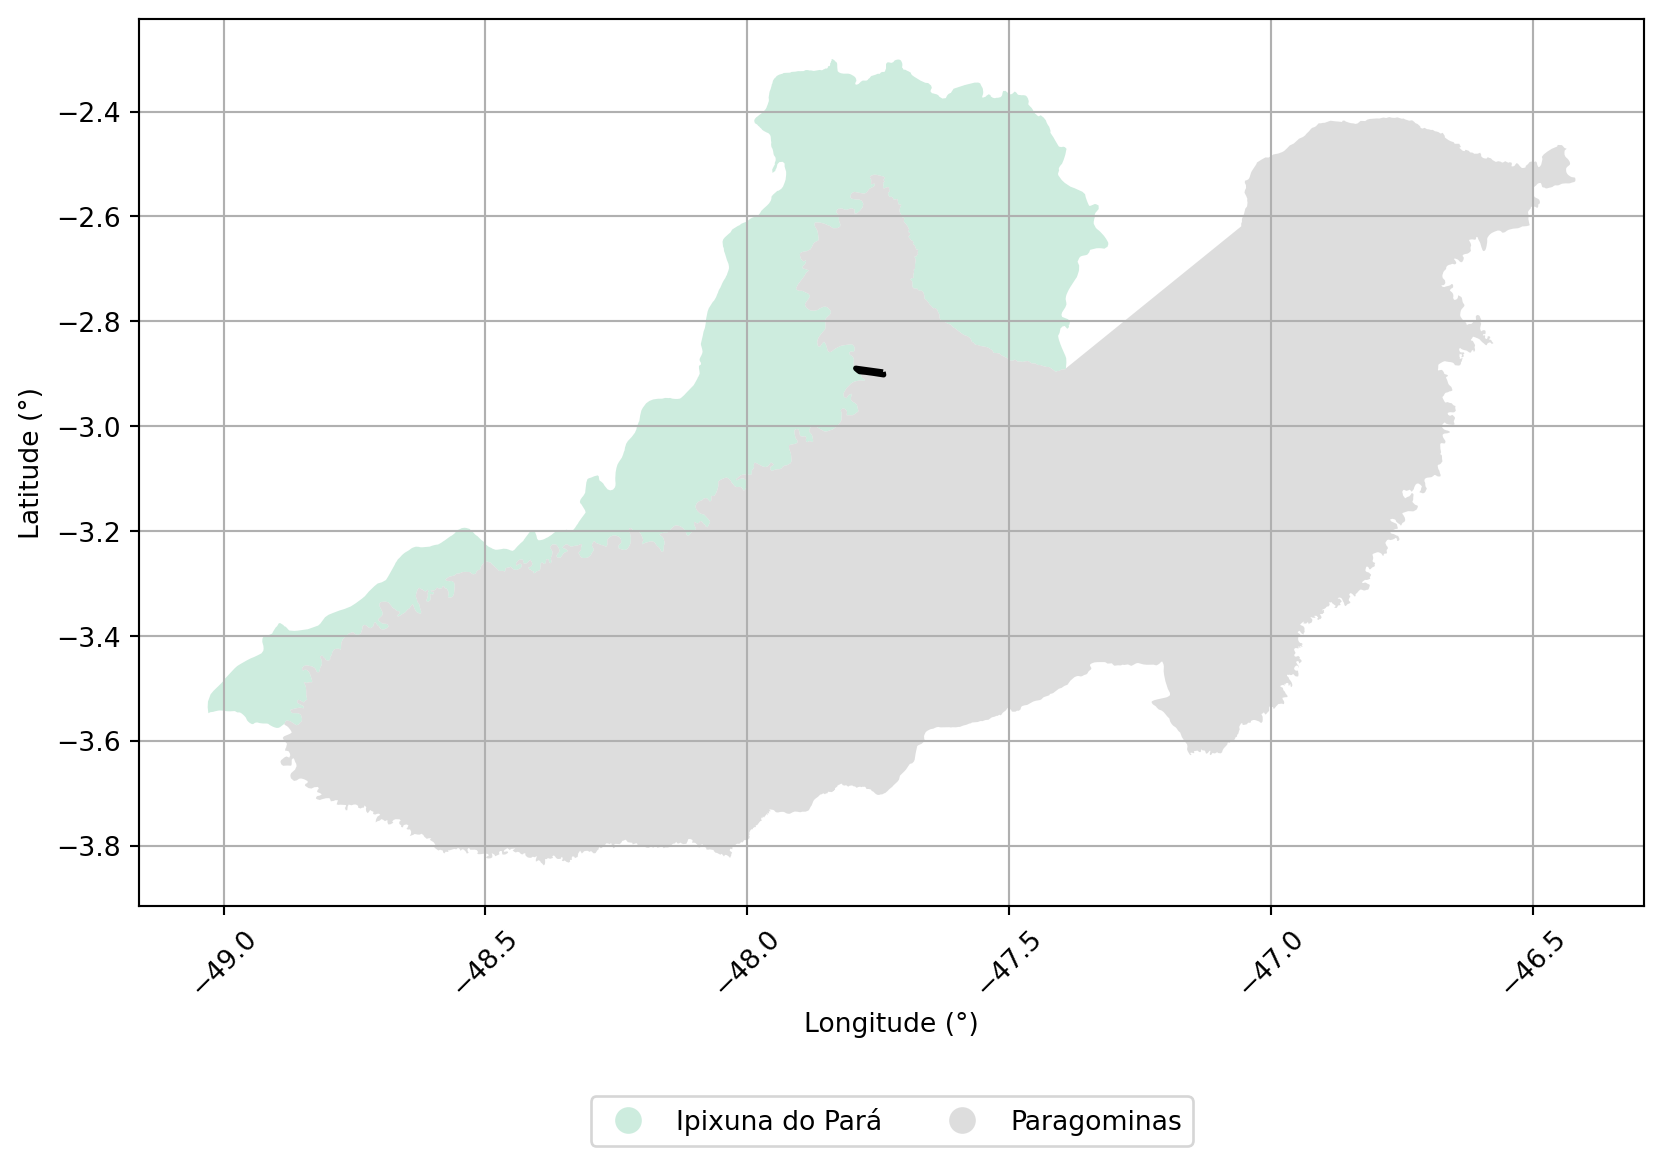
\includegraphics{xx-analise-individual-modelo_files/figure-pdf/cell-3-output-83.pdf}

\n  

\n    

\n      

Nome

\n      

Categoria

\n      

Responsabilidade

\n      

Área Sobreposta (ha)

\n    

\n  

\n  

\n    

\n      

RESERVA EXTRATIVISTA DO CAZUMBÁ-IRACEMA

\n      

Reserva Extrativista

\n      

federal

\n      

28074.8867

\n    

\n  

\n

\subsubsection{Terras Indígenas}\label{terras-induxedgenas-4}

Não há sobreposição

\subsubsection{Projetos de
Assentamento}\label{projetos-de-assentamento-4}

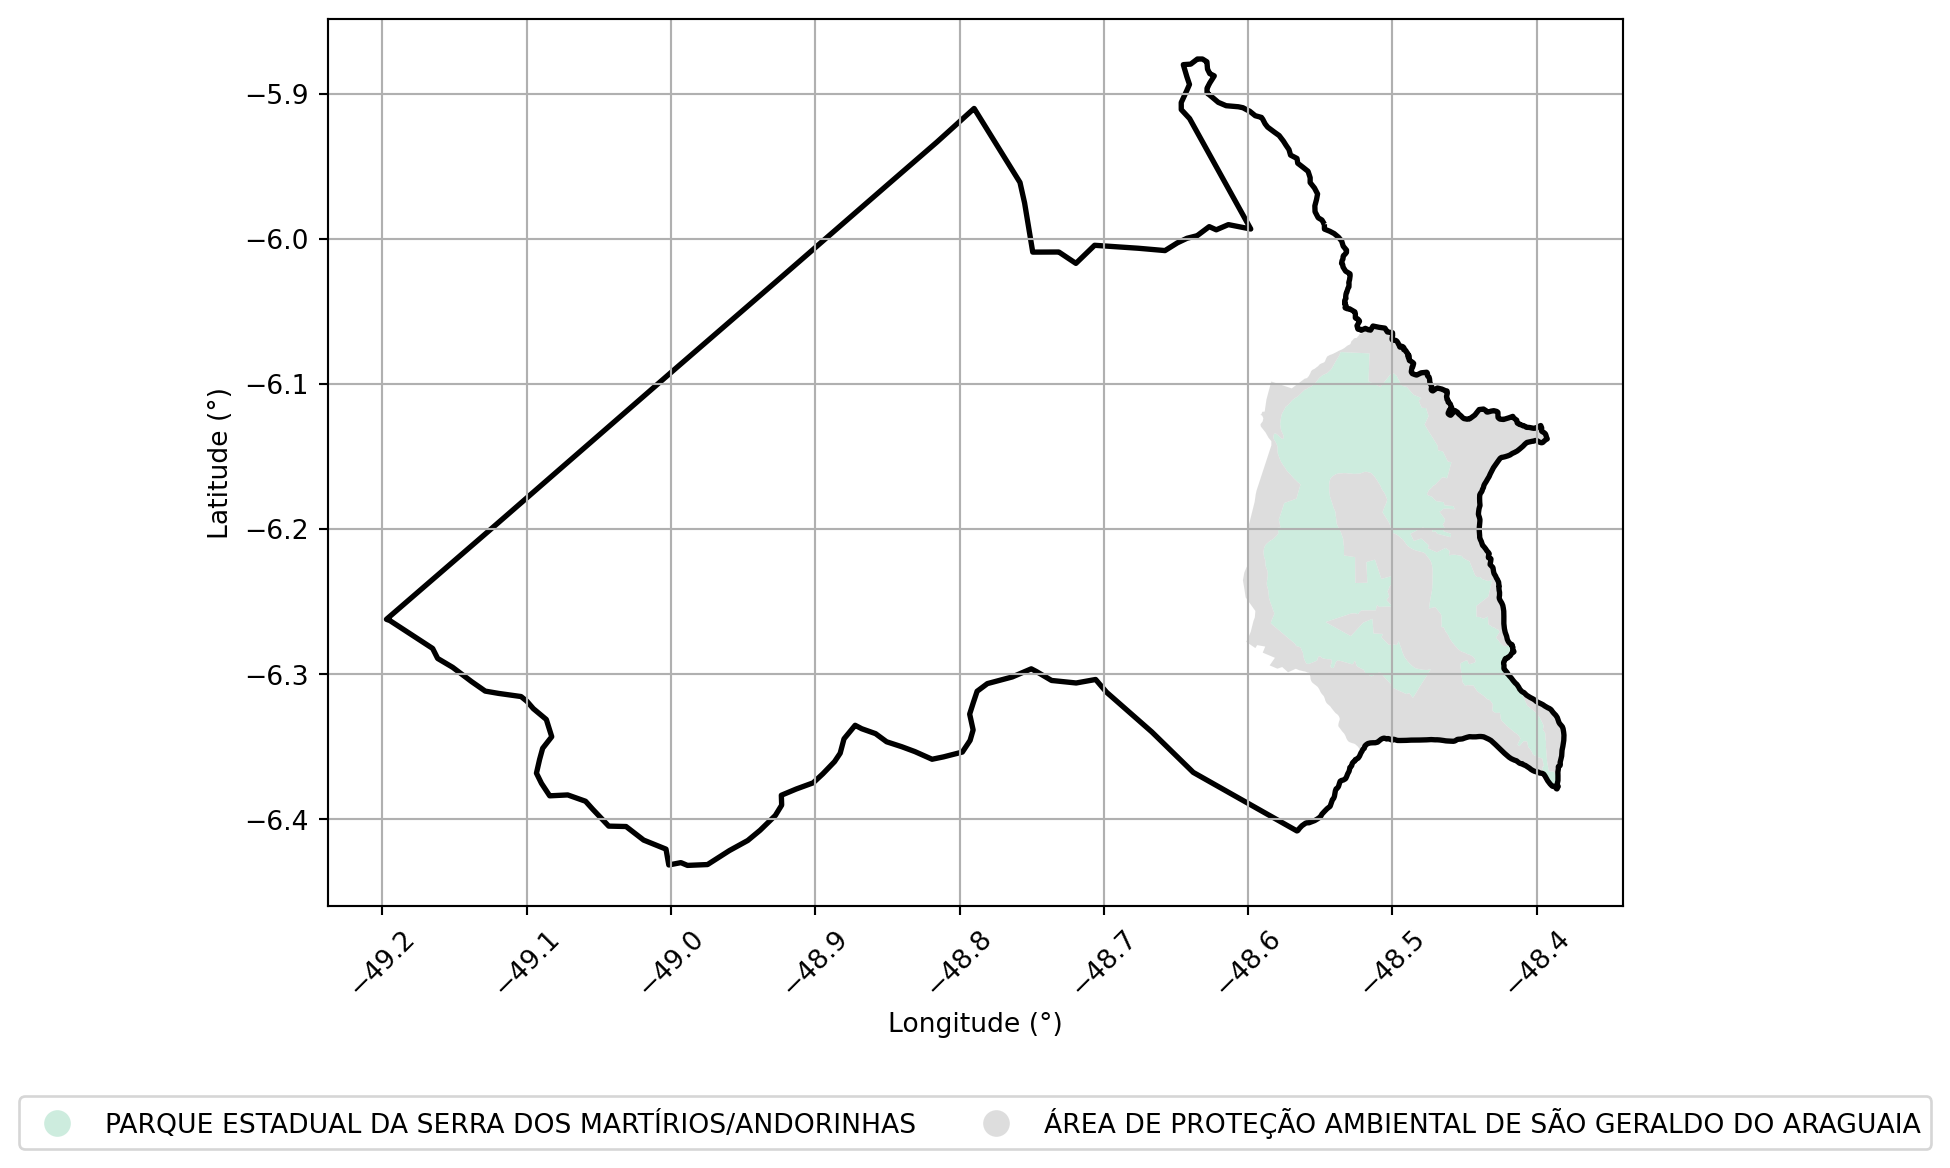
\includegraphics{xx-analise-individual-modelo_files/figure-pdf/cell-3-output-88.pdf}

\n  

\n    

\n      

SIPRA

\n      

Nome

\n      

Município

\n      

Área Sobreposta (ha)

\n    

\n  

\n  

\n    

\n      

AC0096000

\n      

RESEX RESERVA EXTRATIVISTA CAZUMBÁ/IRACEMA

\n      

SENA MADUREIRA

\n      

28013.4795

\n    

\n  

\n

\subsubsection{Território Quilombola}\label{territuxf3rio-quilombola-4}

Não há sobreposição

\subsubsection{SIGEF}\label{sigef-4}

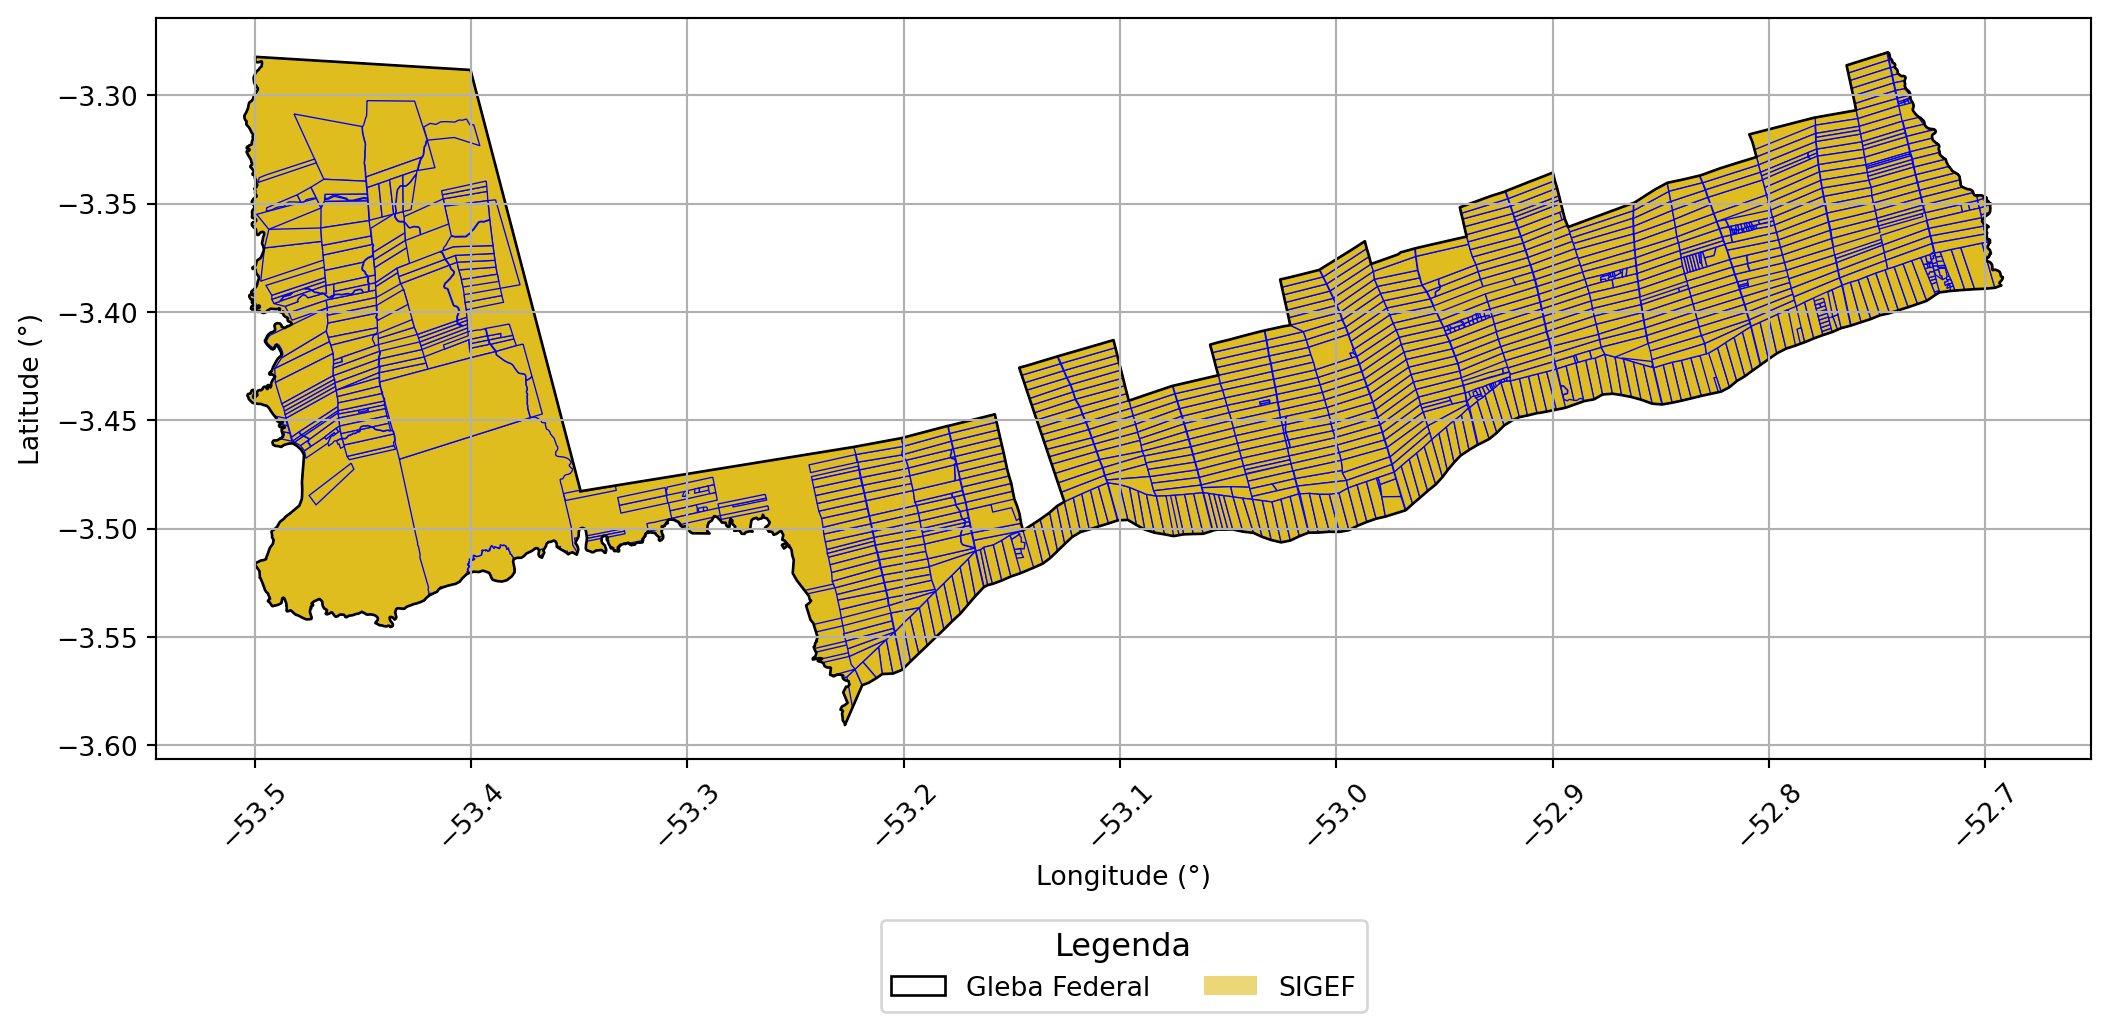
\includegraphics{xx-analise-individual-modelo_files/figure-pdf/cell-3-output-93.pdf}

\n  

\n    

\n      

Código SIGEF

\n      

Natureza do Polígono

\n      

Área Sobreposta (ha)

\n    

\n  

\n  

\n    

\n      

51482b32-2664-4d0e-bcda-38fdcce815df

\n      

Particular

\n      

85.3907

\n    

\n    

\n      

eeb2e98e-2e68-4665-94de-1d5160e82ed9

\n      

Particular

\n      

171.7814

\n    

\n    

\n      

2c165fb2-024c-4e08-989e-f8f27d150acb

\n      

Particular

\n      

200.2304

\n    

\n    

\n      

4d313aef-7694-4ab3-957e-e089ab16c230

\n      

Particular

\n      

351.5850

\n    

\n    

\n      

2fa4e26d-5e75-47ea-bd2a-5f3a42dbf2e6

\n      

Particular

\n      

100.6985

\n    

\n    

\n      

8cfb8db1-8dac-426a-94b0-3548f121a875

\n      

Particular

\n      

995.2632

\n    

\n    

\n      

8ac36740-bcbf-4ac5-8da8-316fde9f52ab

\n      

Particular

\n      

102.9296

\n    

\n    

\n      

51953150-773a-4488-a2ee-4009cbc5fe60

\n      

Particular

\n      

1443.0892

\n    

\n    

\n      

97ab7a28-d4c5-4c6d-ad78-204d26eb7c46

\n      

Particular

\n      

103.0872

\n    

\n    

\n      

9c902c41-7d24-4498-bbd9-2cfbcfb80101

\n      

Particular

\n      

354.1920

\n    

\n    

\n      

447cc703-7a7f-45ce-90d1-570def300791

\n      

Particular

\n      

317.2647

\n    

\n    

\n      

0ea0a497-febb-4051-8a78-8a45fd425473

\n      

Particular

\n      

39.0454

\n    

\n    

\n      

207c7275-82d3-49ec-a849-161954bf492d

\n      

Particular

\n      

16.5042

\n    

\n    

\n      

5a6f61be-3f26-4abf-8fef-8281b4c7b7b4

\n      

Particular

\n      

44.9256

\n    

\n    

\n      

34ebea6a-82bc-4a0a-838d-469cdec6a8c1

\n      

Particular

\n      

421.4599

\n    

\n    

\n      

682f5773-a625-4283-ac73-483fc45e308c

\n      

Particular

\n      

22.6787

\n    

\n    

\n      

7394f86f-35e1-4ac3-9491-59f95698c4b1

\n      

Particular

\n      

151.0903

\n    

\n    

\n      

2ed4ffa5-56f2-4797-ad2e-6f1049c6b231

\n      

Particular

\n      

16.9752

\n    

\n    

\n      

15822da0-4e18-4689-9f3c-f3e8bf6803b6

\n      

Particular

\n      

90.1684

\n    

\n    

\n      

48783c82-c0bc-4d2d-ba80-5154bee70b60

\n      

Particular

\n      

51.7297

\n    

\n    

\n      

e024f2b6-f3db-4a49-a6cd-0971f06d417e

\n      

Particular

\n      

44.4708

\n    

\n    

\n      

e6b46e24-af83-4a59-bccc-58f1780e3611

\n      

Particular

\n      

51.5078

\n    

\n    

\n      

8931db9c-3730-49bf-b4e7-3d05074375ea

\n      

Particular

\n      

62.4983

\n    

\n    

\n      

820354be-1344-493f-a6e1-efa55e53f57f

\n      

Particular

\n      

98.4082

\n    

\n    

\n      

2b17d6e7-f36a-4f1b-a07a-e80fa3a7539e

\n      

Particular

\n      

104.4316

\n    

\n    

\n      

9f94541a-d859-43e1-b9ed-27c416d91bdf

\n      

Particular

\n      

162.6942

\n    

\n    

\n      

27fcd6f6-b8ca-4951-86f5-678748d7e2dd

\n      

Particular

\n      

174.4303

\n    

\n    

\n      

ca340e3e-3ae3-4e42-8354-5d201bd72860

\n      

Particular

\n      

57.3460

\n    

\n    

\n      

dac06bbe-7bfd-4180-8e4b-96de4bb73ce4

\n      

Particular

\n      

54.8222

\n    

\n    

\n      

feb636b0-5478-414b-bca6-ac29605878f8

\n      

Particular

\n      

56.4734

\n    

\n    

\n      

a8fa5f52-b624-4e87-816a-8192d08a27dc

\n      

Particular

\n      

26.7666

\n    

\n    

\n      

d2da493a-4a50-44c2-92db-3adbe4caa7e9

\n      

Particular

\n      

102.9269

\n    

\n    

\n      

c55348f0-a4f5-4248-bc22-6258be769e32

\n      

Particular

\n      

100.5003

\n    

\n    

\n      

883e851e-0c4b-4b18-a633-c8445cf9897e

\n      

Particular

\n      

99.4796

\n    

\n    

\n      

92f45ffd-2ac6-457d-a08c-f8c45c1f69a4

\n      

Particular

\n      

96.2449

\n    

\n    

\n      

e698bf13-ae8f-42fb-944b-3cb23e9e24f9

\n      

Particular

\n      

300.9151

\n    

\n    

\n      

0c1258a0-cf00-4d37-be44-5f976156c425

\n      

Particular

\n      

101.8767

\n    

\n    

\n      

2ab00dd4-b8f8-40a5-a71f-7bb07f44fedf

\n      

Particular

\n      

491.2597

\n    

\n    

\n      

e592ff51-b085-439d-ac5a-25efd779586e

\n      

Particular

\n      

101.7647

\n    

\n    

\n      

9554423a-404b-465d-8ee0-1731168496cf

\n      

Particular

\n      

98.2770

\n    

\n    

\n      

f962ac52-c0e6-472c-814b-e231b952bedc

\n      

Particular

\n      

186.8252

\n    

\n    

\n      

7f04a9bf-b8d1-4a59-8f2a-d0c616b3fcac

\n      

Particular

\n      

1310.3839

\n    

\n    

\n      

c531687c-e49d-4856-b2ff-d8916b47fc45

\n      

Particular

\n      

91.7304

\n    

\n    

\n      

963997e5-82e7-47f3-8c2f-a33560d6a173

\n      

Particular

\n      

92.5987

\n    

\n    

\n      

ee1d6140-9ed9-49bb-9d49-3bb5f5948103

\n      

Particular

\n      

159.1096

\n    

\n    

\n      

8d1f1f3f-adc3-42a4-8533-89f30b131716

\n      

Particular

\n      

92.6003

\n    

\n    

\n      

eb4e60e5-5e89-4920-9cf6-ba97f696ef0b

\n      

Particular

\n      

64.5631

\n    

\n    

\n      

fb64ab0a-6d77-4b53-8f70-2457d50d0e00

\n      

Particular

\n      

28.9195

\n    

\n    

\n      

5628f143-a972-4959-9a6b-7a90a0e921e8

\n      

Particular

\n      

55.3712

\n    

\n    

\n      

f93b6b3e-a6cf-4500-bda6-dda91be2ec27

\n      

Particular

\n      

73.8856

\n    

\n    

\n      

1d88c69b-ccb5-43f6-9cde-415444cbda2b

\n      

Particular

\n      

75.0791

\n    

\n    

\n      

ae2a8019-96b0-4530-a11c-e0a66bcf6966

\n      

Particular

\n      

207.9254

\n    

\n    

\n      

3d8f03c4-9e71-4a59-88de-ce9e92f8c974

\n      

Particular

\n      

32.3153

\n    

\n    

\n      

2942b642-cc15-4f02-9382-07989da9dc1c

\n      

Particular

\n      

57.1145

\n    

\n    

\n      

96b8d4d2-13eb-48a4-b2fd-99c268540c77

\n      

Particular

\n      

80.9297

\n    

\n    

\n      

93c3b595-9eea-41b0-bc13-a1472765da44

\n      

Particular

\n      

60.7697

\n    

\n    

\n      

eb5b50e8-0131-45a0-9b01-18c9f5c18ab0

\n      

Particular

\n      

92.5350

\n    

\n    

\n      

3fd03714-4b63-4b65-95f5-c844069a99b4

\n      

Particular

\n      

93.0662

\n    

\n    

\n      

1191cf66-6a82-4a2d-b70e-70b38ee41cbc

\n      

Particular

\n      

56.1242

\n    

\n    

\n      

65fa2f9c-cd12-45c1-a232-599f95a7986e

\n      

Particular

\n      

73.3664

\n    

\n    

\n      

00636b9f-eba5-4473-b311-c38a1e5f7cf2

\n      

Particular

\n      

52.8522

\n    

\n    

\n      

338bec34-9309-49f8-af3d-d7c83ba3c286

\n      

Particular

\n      

77.5910

\n    

\n    

\n      

7a3e4275-7a9a-4e97-ba53-c8ce685cebcb

\n      

Particular

\n      

92.7472

\n    

\n    

\n      

3212d413-55ce-4129-bcbc-e04caa13e90d

\n      

Particular

\n      

93.5491

\n    

\n    

\n      

c7d2cfdc-43f5-4d58-a6c4-331731f4e1e0

\n      

Particular

\n      

73.1315

\n    

\n    

\n      

abd8a682-adbe-45f9-94e2-22077c33dad7

\n      

Particular

\n      

192.0074

\n    

\n    

\n      

0dc5b8b3-d37d-4874-aabd-09e295b76189

\n      

Particular

\n      

92.5940

\n    

\n    

\n      

45fe781a-d82d-4a83-b5ed-8595d7c3f401

\n      

Particular

\n      

116.7512

\n    

\n    

\n      

f9326481-22b2-4256-a0b9-ee6fd99ed9c4

\n      

Particular

\n      

77.4232

\n    

\n    

\n      

dad76f5b-d720-403e-a45f-8fb929cbba1b

\n      

Particular

\n      

69.4968

\n    

\n    

\n      

aa96e043-9f5f-4c88-803b-f2a8588d790b

\n      

Particular

\n      

115.4270

\n    

\n    

\n      

5ffa1836-6c26-467b-ba7d-066f74f6eddf

\n      

Particular

\n      

124.4089

\n    

\n    

\n      

62917672-b43e-41a4-9657-10a4bf5ce303

\n      

Particular

\n      

125.8993

\n    

\n    

\n      

f422a3b2-59d4-4540-b334-55e99701d4a3

\n      

Particular

\n      

71.2640

\n    

\n    

\n      

8aa39b2b-3bcd-4bfc-a367-0985a68ebd27

\n      

Particular

\n      

45.4304

\n    

\n    

\n      

79b3b67c-db51-48f7-a628-0308db9b4842

\n      

Particular

\n      

195.5996

\n    

\n    

\n      

53132944-bedc-4dcc-8e27-c141aa11ea3c

\n      

Particular

\n      

70.5908

\n    

\n    

\n      

8681dad0-abfd-47b7-a531-e8f3b4b1ed43

\n      

Particular

\n      

261.4605

\n    

\n    

\n      

3e5039d1-4f7a-41e4-a1cf-f6906c005965

\n      

Particular

\n      

83.8110

\n    

\n    

\n      

23b34225-65e1-4380-ba25-7d667b9fb6bb

\n      

Particular

\n      

76.1812

\n    

\n    

\n      

b4eca7b8-d846-44d3-aad5-233cf4b91434

\n      

Particular

\n      

93.0367

\n    

\n    

\n      

bf531381-15ea-48d5-b9c8-6ac5a20cbec8

\n      

Particular

\n      

80.0988

\n    

\n    

\n      

2d2201cd-bb22-460c-92d6-02b0f56c3ad5

\n      

Particular

\n      

119.6783

\n    

\n    

\n      

bcdac28e-8086-4def-9495-754a11a67fb8

\n      

Particular

\n      

103.2167

\n    

\n    

\n      

83dab21e-02bd-46c9-899f-7923bfcd819c

\n      

Particular

\n      

99.7008

\n    

\n    

\n      

c43122cb-6c70-4aa2-bfed-439c420bf1c7

\n      

Particular

\n      

94.9328

\n    

\n    

\n      

fd3c8d69-a1df-46a1-ac6a-9be40d0029a8

\n      

Particular

\n      

1025.1605

\n    

\n    

\n      

89d97015-a77c-4068-b35b-d069c54d1c2d

\n      

Particular

\n      

2507.7625

\n    

\n    

\n      

c8bda508-05e5-464e-a6cf-2f7b2ebf695d

\n      

Particular

\n      

144.5645

\n    

\n    

\n      

4da1e3c7-1d52-4df5-9f65-27c91ac138a5

\n      

Particular

\n      

1083.2067

\n    

\n    

\n      

f2636b40-a8a1-4b28-8735-e9c7a22ada79

\n      

Particular

\n      

1092.6003

\n    

\n    

\n      

bbb13fe0-e04f-4a4b-9409-a80482c91175

\n      

Particular

\n      

90.4850

\n    

\n    

\n      

888d8e71-ecdb-47ce-861d-1de23d7eb6d6

\n      

Particular

\n      

92.5192

\n    

\n    

\n      

efef5080-4ab6-4005-a3ec-91751532d51e

\n      

Particular

\n      

78.1367

\n    

\n    

\n      

6843fb3f-4fb9-44ea-8ccd-311cb13b00ba

\n      

Particular

\n      

151.5695

\n    

\n    

\n      

cd536b31-1dc5-4226-a71a-55609aae3c17

\n      

Unidade de Conservação

\n      

22.4281

\n    

\n  

\n

\subsubsection{SNCI}\label{snci-4}

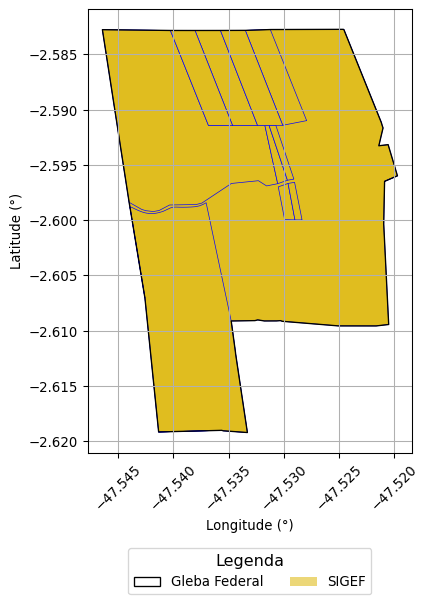
\includegraphics{xx-analise-individual-modelo_files/figure-pdf/cell-3-output-96.pdf}

\n  

\n    

\n      

Código SNCI

\n      

Área Sobreposta (ha)

\n    

\n  

\n  

\n    

\n      

140712000001-40

\n      

0.1599

\n    

\n    

\n      

141109000002-87

\n      

66868.9887

\n    

\n  

\n

\subsection{Gleba Analisada: BOA ESPERANÇA
I}\label{gleba-analisada-boa-esperanuxe7a-i}

\n  

\n    

\n      

Nome da Gleba

\n      

Área (ha)

\n    

\n  

\n  

\n    

\n      

BOA ESPERANÇA I

\n      

890.1892

\n    

\n  

\n

\subsubsection{Abrangência Municipal}\label{abranguxeancia-municipal-5}

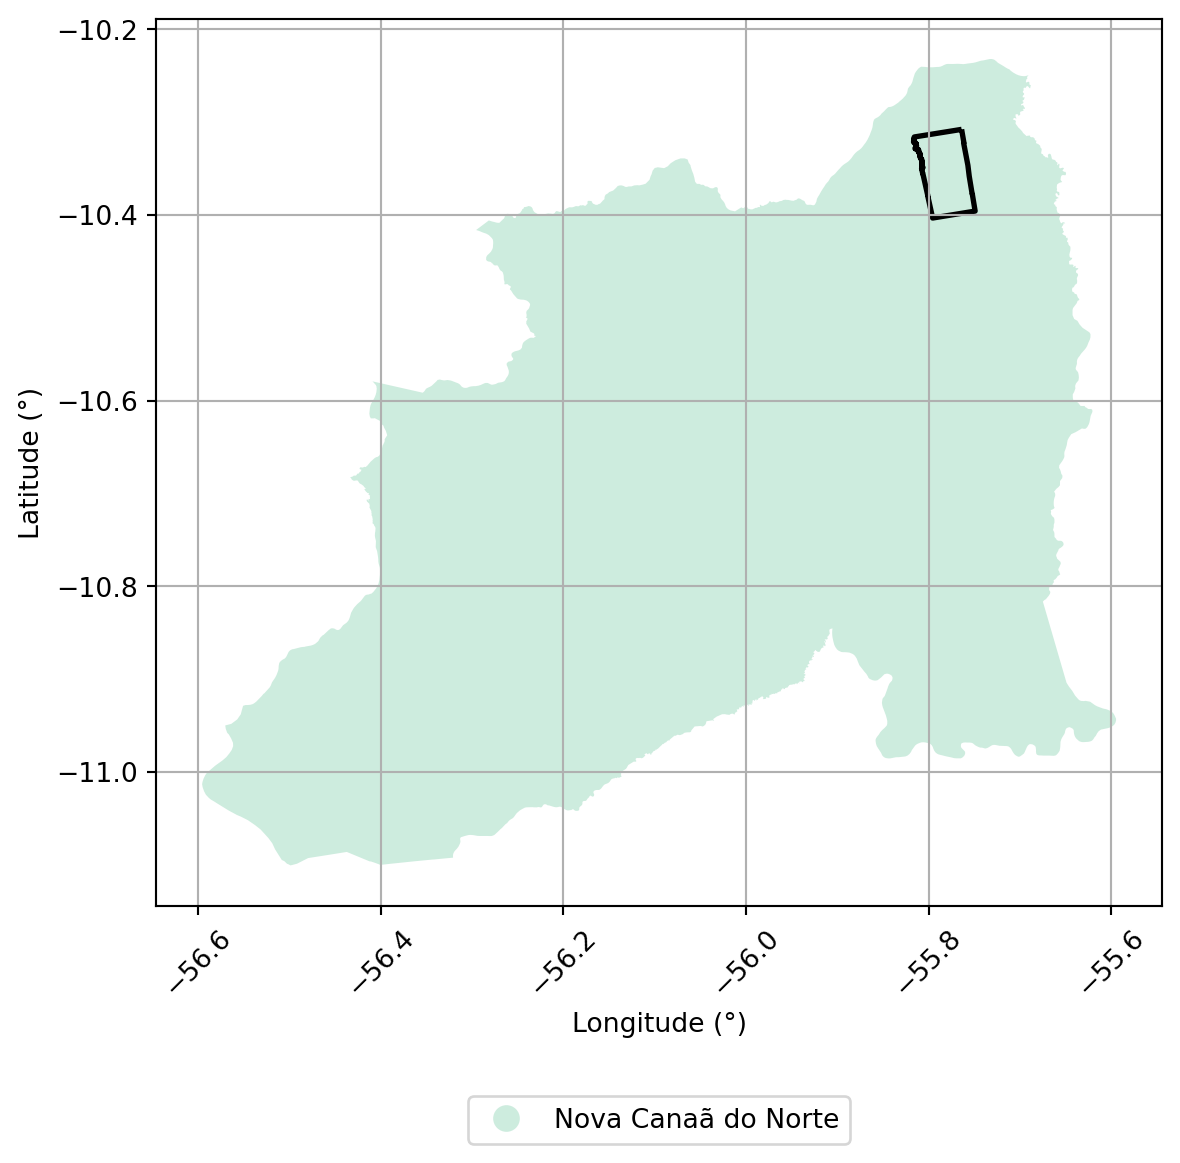
\includegraphics{xx-analise-individual-modelo_files/figure-pdf/cell-3-output-101.pdf}

\n  

\n    

\n      

Código da UF

\n      

Estado

\n      

UF

\n      

Código do Município

\n      

Nome do Município

\n    

\n  

\n  

\n    

\n      

12.0000

\n      

Acre

\n      

AC

\n      

1200609

\n      

Tarauacá

\n    

\n  

\n

\subsubsection{Unidades de
Conservação}\label{unidades-de-conservauxe7uxe3o-5}

Não há sobreposição

\subsubsection{Terras Indígenas}\label{terras-induxedgenas-5}

Não há sobreposição

\subsubsection{Projetos de
Assentamento}\label{projetos-de-assentamento-5}

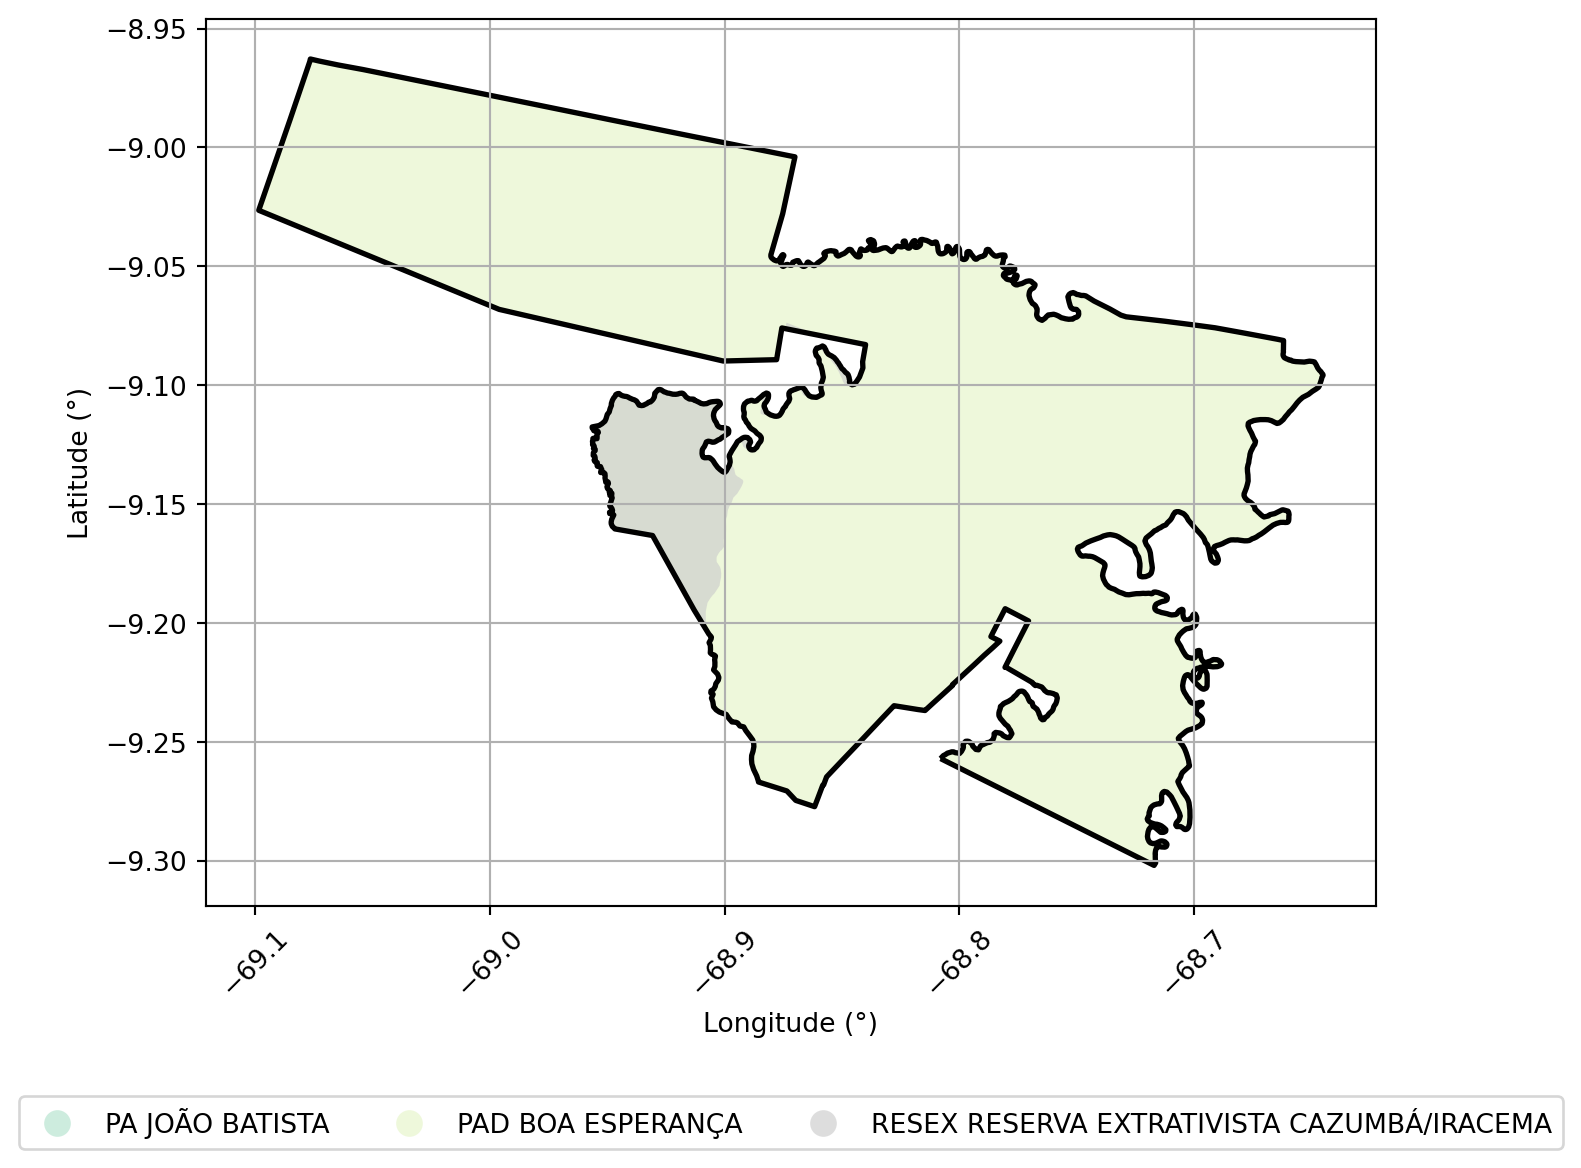
\includegraphics{xx-analise-individual-modelo_files/figure-pdf/cell-3-output-108.pdf}

\n  

\n    

\n      

SIPRA

\n      

Nome

\n      

Município

\n      

Área Sobreposta (ha)

\n    

\n  

\n  

\n    

\n      

AC0047000

\n      

PA TARAUACÁ

\n      

TARAUACA

\n      

0.1242

\n    

\n  

\n

\subsubsection{Território Quilombola}\label{territuxf3rio-quilombola-5}

Não há sobreposição

\subsubsection{SIGEF}\label{sigef-5}

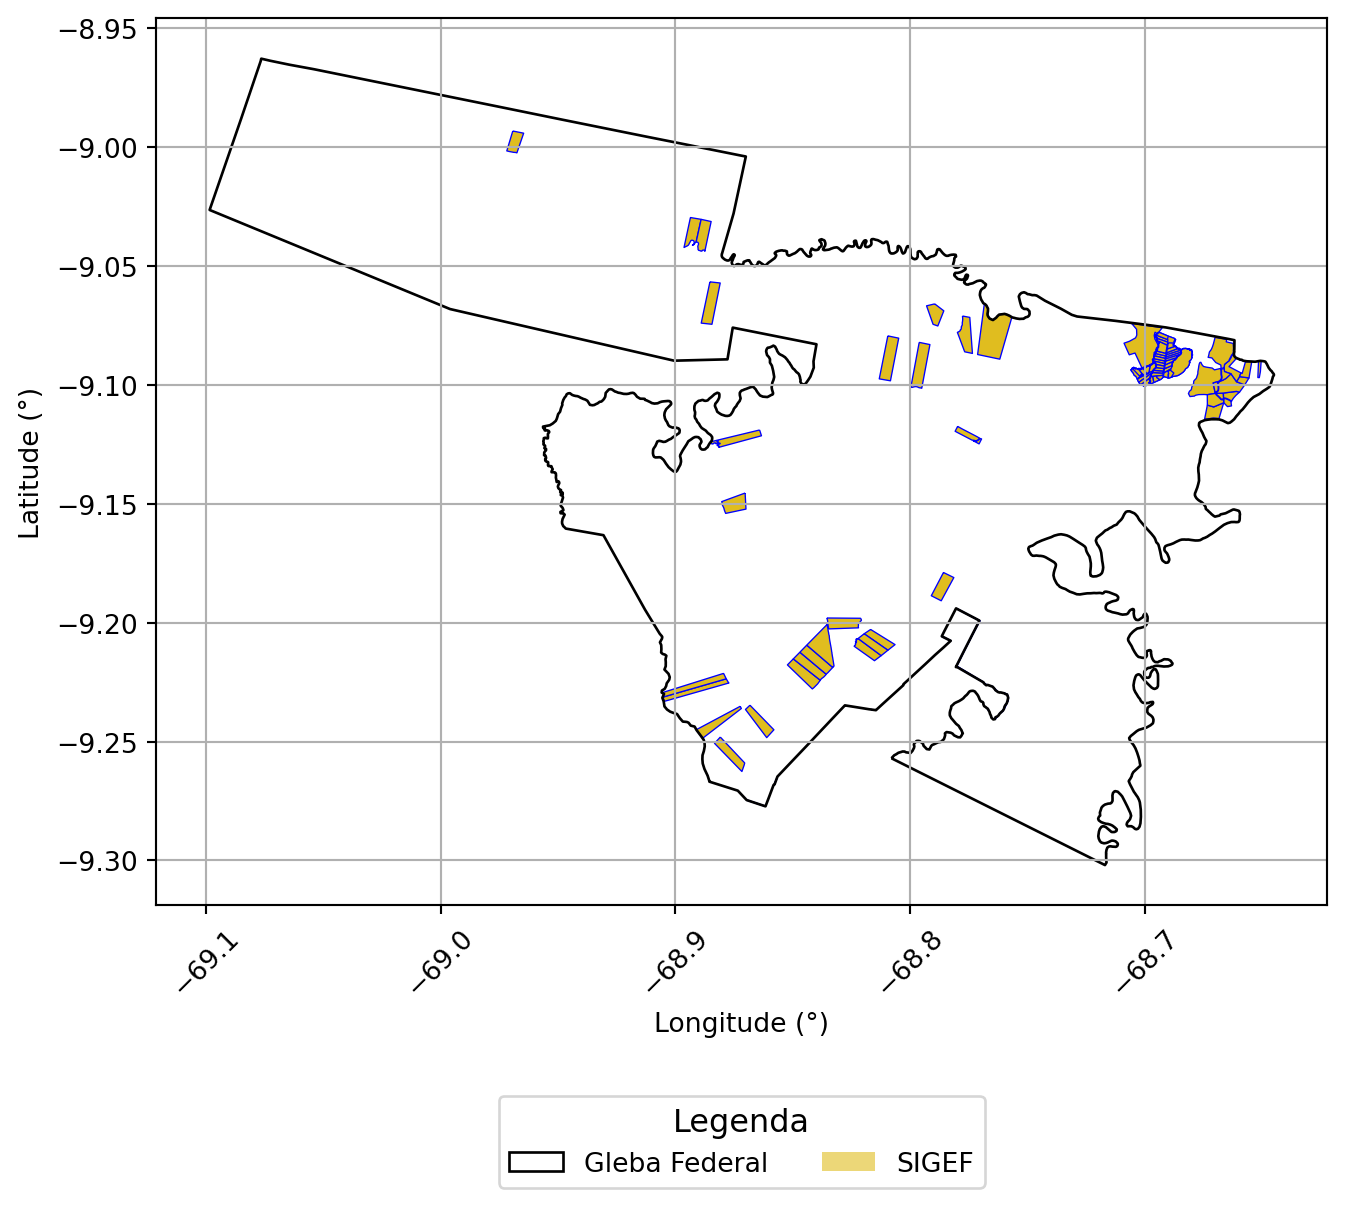
\includegraphics{xx-analise-individual-modelo_files/figure-pdf/cell-3-output-113.pdf}

\n  

\n    

\n      

Código SIGEF

\n      

Natureza do Polígono

\n      

Área Sobreposta (ha)

\n    

\n  

\n  

\n    

\n      

e3685821-5c7f-4d58-9296-75f2d822d1d8

\n      

Gleba Pública

\n      

0.0068

\n    

\n    

\n      

8120d76b-c635-4107-9440-c31879275dfe

\n      

Particular

\n      

0.0000

\n    

\n    

\n      

5c35fd89-2da5-4c5d-819d-32874d070eaf

\n      

Particular

\n      

0.0000

\n    

\n    

\n      

f2e69c4e-ae18-41f6-a3ef-d6b06c747b7f

\n      

Particular

\n      

0.0000

\n    

\n    

\n      

2dc5ca4a-b5cf-4ea5-b1af-8ceb4f50dcc2

\n      

Particular

\n      

0.0000

\n    

\n    

\n      

edbfa15d-d2c7-4997-bd60-845fb7173f37

\n      

Particular

\n      

0.0000

\n    

\n    

\n      

746604e7-fccb-4801-9ed8-fcef0a68f35c

\n      

Particular

\n      

0.0000

\n    

\n    

\n      

6b7e5f44-b27d-4858-8ff2-63b789f86bab

\n      

Particular

\n      

103.1388

\n    

\n    

\n      

d6305744-6698-4c12-a442-3e21fbb3236c

\n      

Particular

\n      

82.3547

\n    

\n    

\n      

82425e62-1eb0-4a56-a61a-f3e2451be766

\n      

Particular

\n      

100.1469

\n    

\n    

\n      

4b099726-a071-4bc2-8c99-09c26eb4ee3e

\n      

Particular

\n      

17.6199

\n    

\n    

\n      

b2983919-f1f4-483c-82f1-bb17cef72764

\n      

Particular

\n      

96.4014

\n    

\n    

\n      

0d8387a2-3124-49fd-94f4-0e5962ef1b4b

\n      

Particular

\n      

101.9050

\n    

\n  

\n

\subsubsection{SNCI}\label{snci-5}

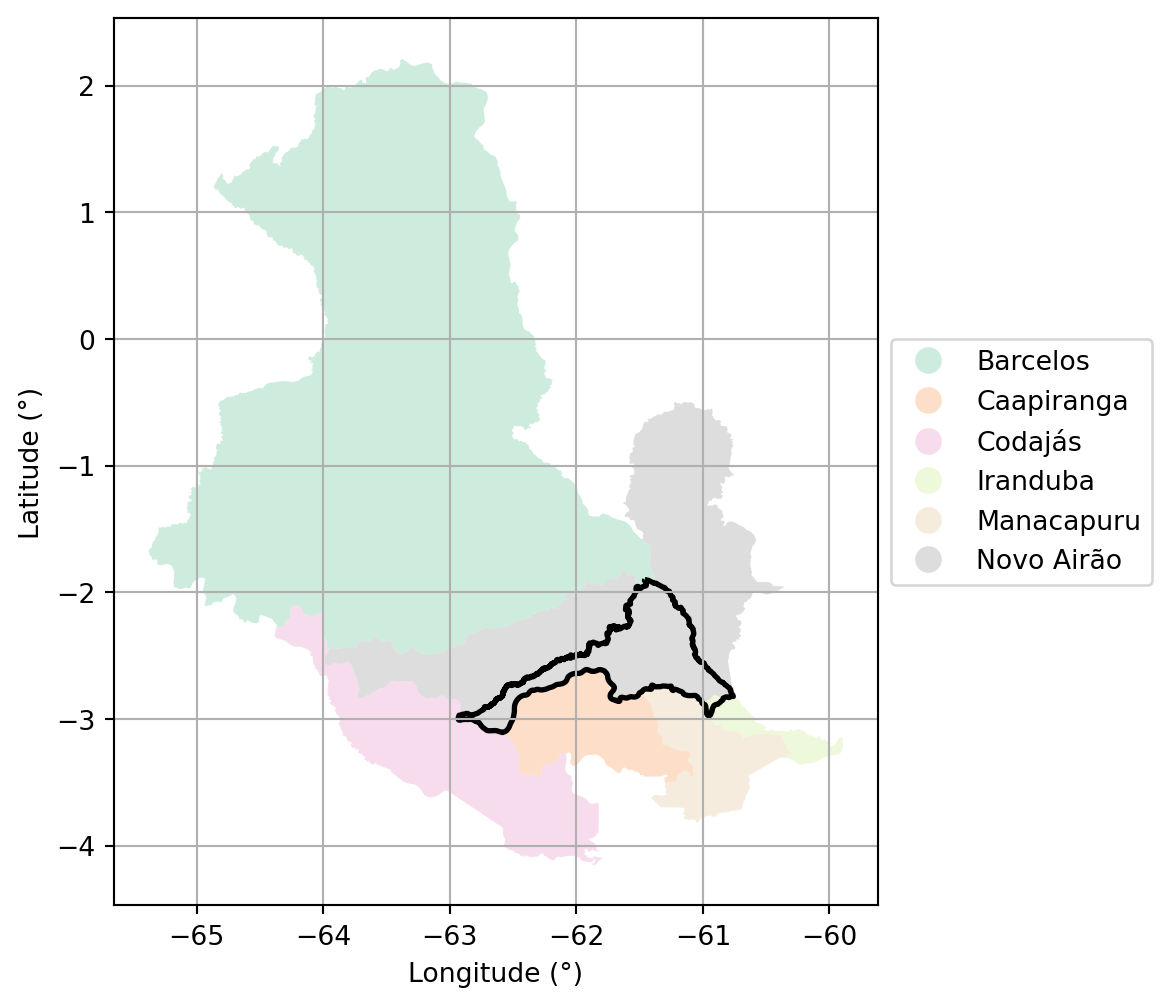
\includegraphics{xx-analise-individual-modelo_files/figure-pdf/cell-3-output-116.pdf}

\n  

\n    

\n      

Código SNCI

\n      

Área Sobreposta (ha)

\n    

\n  

\n  

\n    

\n      

141612000003-00

\n      

0.0301

\n    

\n    

\n      

141612000004-83

\n      

0.0116

\n    

\n    

\n      

141612000002-11

\n      

0.0606

\n    

\n  

\n



\end{document}
